\documentclass[a4paper, 12pt]{article}
\usepackage[left=2.5cm, right=2.5cm, top=3cm, bottom=3cm]{geometry}
\usepackage[spanish]{babel}
\usepackage{amsmath}
\usepackage{graphicx}
\usepackage{color}
\usepackage{xcolor}
\usepackage[utf8]{inputenc}
\usepackage[T1]{fontenc}
\usepackage{listings}
\usepackage{tikz}
\usetikzlibrary{shapes,arrows,positioning}

\definecolor{colorgreen}{rgb}{0,0.6,0}
\definecolor{colorgray}{rgb}{0.5,0.5,0.5}
\definecolor{colorpurple}{rgb}{0.58,0,0.82}
\definecolor{colorback}{RGB}{255,255,204}
\definecolor{colorbackground}{RGB}{200,200,221}
%Definiendo el estilo de las porciones de codigo
\lstset{
 backgroundcolor=\color{colorbackground},
commentstyle=\color{colorgreen},
keywordstyle=\color{colorpurple},
numberstyle=\tiny\color{colorgray},
stringstyle=\color{colorgreen},
basicstyle=\ttfamily\footnotesize,
breakatwhitespace=false,
breaklines=true,
captionpos=b,
keepspaces=true,
numbers=left,
showspaces=false,
showstringspaces=false,
showtabs=false,
tabsize=2,
frame=single,
framesep=2pt,
rulecolor=\color{black},
framerule=1pt
}



\begin{document}
\graphicspath{{./}}

\begin{center}
\text{\huge \textbf{Informe del Proyecto Final} }\\
\vspace {0.5cm}
\text{\huge \textbf{de}}\\
\vspace {0.5cm}
\text{\huge \textbf{Estadística}}\\
\vspace {5cm}
\text{\huge Richard Alejandro Matos Arderí}\\
\text{\huge Mauricio Sunde Jiménez}\\
\vspace {1cm}
\vspace {2cm}
\text{\Large Grupo 311, Ciencia de la Computación.}\\
\vspace {0.5cm}
\text{\Large Facultad de Matemática y Computación}\\
\text{\Large Universidad de La Habana.}\\
\vspace {0.5cm}
\begin{figure}[h]
    \centering
    
\includegraphics[width=0.2\textwidth, height=0.2\textheight]{MATCOM.jpg}
\end{figure}
\vspace {0.5cm}
\text{2024}\\


\end{center}

\newpage
\tableofcontents
\newpage

\section{Introducción}

 Este proyecto de análisis estadístico, realizado como parte del plan de estudios de Ciencia de la Computación, se centra en el conjunto de datos \textbf{Breast Cancer Wisconsin (Diagnostics)}. Este dataset, ampliamente utilizado en la investigación de aprendizaje automático y análisis de datos biomédicos, contiene información crucial para la clasificación de tumores mamarios como benignos o malignos. Nuestro objetivo es ir más allá de una simple clasificación y profundizar en un análisis estadístico exhaustivo, explorando las características de los datos y sus relaciones intrínsecas.\\

En una primera etapa, emplearemos técnicas de estadística descriptiva para obtener una comprensión inicial del dataset. Esto incluirá el cálculo de medidas de tendencia central (media, mediana, moda) y medidas de dispersión (desviación estándar, varianza, rango intercuartílico) para cada variable, proporcionando una visión general de la distribución de los datos. Además, analizaremos la curtosis para determinar la forma de las distribuciones y la presencia de valores atípicos.\\

Posteriormente, nos adentraremos en el ámbito de la estadística inferencial. Comenzaremos con la estimación puntual y por intervalos de confianza de parámetros clave, como la media y la proporción, para inferir características de la población a partir de la muestra disponible. Realizaremos pruebas de normalidad (Shapiro-Wilk, Kolmogorov-Smirnov) para determinar si las distribuciones de las variables se ajustan a una distribución normal, un requisito para muchas pruebas paramétricas. Además, llevaremos a cabo pruebas de hipótesis sobre los parámetros de la población, examinando si existen diferencias significativas entre los grupos de tumores benignos y malignos.\\

Un aspecto fundamental de este proyecto será el análisis de las relaciones entre variables. Emplearemos técnicas de análisis de correlación (Pearson, Spearman) para identificar la fuerza y dirección de la asociación entre las características del tumor. También realizaremos pruebas de independencia de variables (chi-cuadrado) para evaluar si existe una relación estadísticamente significativa entre variables categóricas. Finalmente, exploraremos pruebas de homogeneidad para comparar la distribución de variables entre diferentes grupos, contribuyendo a una comprensión más profunda de las diferencias entre tumores benignos y malignos.\\

En resumen, este proyecto pretende ofrecer un análisis estadístico completo y riguroso del dataset \textbf{Breast Cancer Wisconsin (Diagnostics)}, utilizando una variedad de técnicas descriptivas e inferenciales para extraer información relevante y contribuir a una mejor comprensión de las características y relaciones entre los atributos de los tumores mamarios. Los resultados obtenidos permitirán una mejor comprensión de los datos y podrán servir como base para futuros análisis y modelos predictivos.\\

\newpage

\section{Análisis Descriptivo de los datos}

A continuación se muestra un cuadro con todas las variables presentes en el dataset, de conjunto con su clasificación estadística y su escala de medición.
\begin{center}
	

        \begin{tabular}{|p{3.5cm}|p{5.5cm}|p{3cm}|p{2.5cm}|}
            \hline
            \textbf{Variable} & \textbf{Descripción} & \textbf{Clasificación Estadística} & \textbf{Escala de Medición} \\
            \hline
            ID & Identificador único del paciente & Cualitativa & Nominal \\
            
            \textcolor{red}{diagnosis} & Diagnóstico del tumor (1 = maligno, 0 = benigno) & Cualitativa & Nominal \\
            
            \textcolor{red}{radius\_mean} & Radio medio de las células del tumor en $\mu$m & Continua & Razón \\
            
            \textcolor{red}{texture\_mean} & Textura media de las células del tumor & Continua & Razón \\
            
            \textcolor{red}{perimeter\_mean} & Perímetro medio de las células del tumor en $\mu$m & Continua & Razón \\
            
            \textcolor{red}{area\_mean} & Área media de las células del tumor en $\mu$m² & Continua & Razón \\
            
            \textcolor{red}{smoothness\_mean} & Suavidad media de las células del tumor & Continua & Razón \\
            
            \textcolor{red}{compactness\_mean} & Compacidad media de las células del tumor & Continua & Razón \\
            
            concavity\_mean & Concavidad media de las células del tumor & Continua & Razón \\
            
            concave points\_mean & Puntos cóncavos medios de las células del tumor & Continua & Razón \\
            
            \textcolor{red}{symmetry\_mean} & Simetría media de las células del tumor & Continua & Razón \\
            
            fractal dimension\_mean & Dimensión fractal media de las células del tumor & Continua & Razón \\
            
            radius\_se & Desviación estándar del radio de las células del tumor & Continua & Razón \\
            
            texture\_se & Desviación estándar de la textura de las células del tumor & Continua & Razón \\
            
            perimeter\_se & Desviación estándar del perímetro de las células del tumor & Continua & Razón \\
            
            area\_se & Desviación estándar del área de las células del tumor & Continua & Razón \\
            
            smoothness\_se & Desviación estándar de la suavidad de las células del tumor & Continua & Razón \\
            
            compactness\_se & Desviación estándar de la compacidad de las células del tumor & Continua & Razón \\
            \hline
            
        \end{tabular}
        
        \begin{tabular}{|p{3.5cm}|p{5.5cm}|p{3cm}|p{2.5cm}|}
        \hline
            
            concavity\_se & Desviación estándar de la concavidad de las células del tumor & Continua & Razón \\
            
            concave points\_se & Desviación estándar de los puntos cóncavos de las células del tumor & Continua & Razón \\
            
        
            
            symmetry\_se & Desviación estándar de la simetría de las células del tumor & Continua & Razón \\
            
            fractal dimension\_se & Desviación estándar de la dimensión fractal de las células del tumor & Continua & Razón \\
            
            
            \textcolor{red}{radius\_worst} & Radio máximo de las células del tumor en $\mu$m & Continua & Razón \\
            
            \textcolor{red}{texture\_worst} & Textura máxima de las células del tumor & Continua & Razón \\
     
            
            \textcolor{red}{perimeter\_worst} & Perímetro máximo de las células del tumor en $\mu$m & Continua & Razón \\
            
            \textcolor{red}{area\_worst} & Área máxima de las células del tumor en $\mu$m² & Continua & Razón \\
            
            \textcolor{red}{smoothness\_worst} & Suavidad máxima de las células del tumor & Continua & Razón \\
            
            \textcolor{red}{compactness\_worst} & Compacidad máxima de las células del tumor & Continua & Razón \\
            
            concavity\_worst & Concavidad máxima de las células del tumor & Continua & Razón \\
            
            concave points\_worst & Puntos cóncavos máximos de las células del tumor & Continua & Razón \\
            
            \textcolor{red}{symmetry\_worst} & Simetría máxima de las células del tumor & Continua & Razón \\
            
            fractal dimension\_worst & Dimensión fractal máxima de las células del tumor & Continua & Razón \\
            \hline
        \end{tabular}
       
\end{center}


 
Se brindará especial atención a las variables en rojo para el análisis. A continuación se expone una caracterización más detallada de las mismas.


\subsection*{\underline{diagnosis}}

 \begin{itemize}
	\item \textit{Descripción:} Variable categórica que indica si el tumor es maligno o benigno.
	\item \textit{Valores posibles:}
	$1$ (Maligno), $0$ (Benigno).
	\item \textit{Medición:} Determinado a partir del análisis histopatológico.
\end{itemize}

	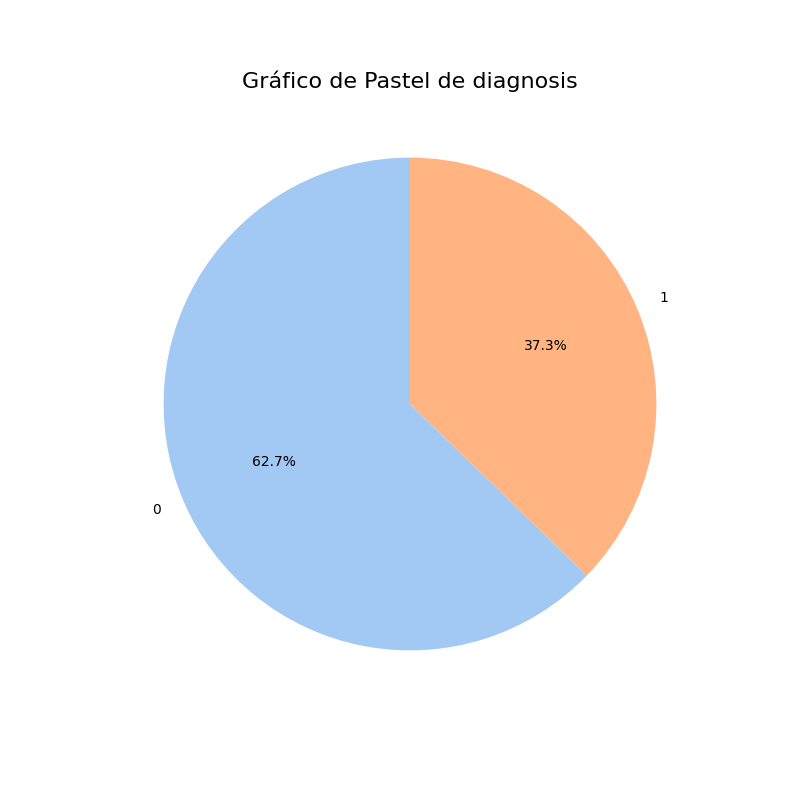
\includegraphics[width=\textwidth]{../Plots/plots_stats/diagnosis/grafico_pastel_diagnosis.png}



	
	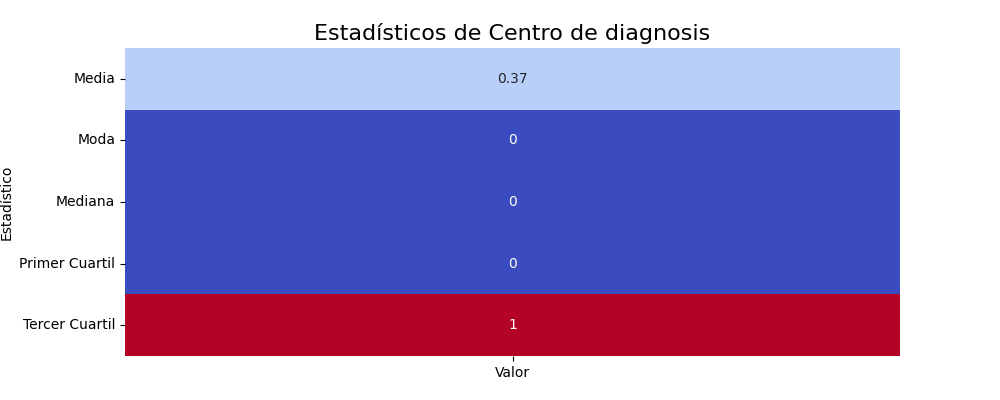
\includegraphics[width=\textwidth]{../Plots/plots_stats/diagnosis/estadisticas_centro_diagnosis.png}




	\includegraphics[width=\textwidth]{../Plots/plots_stats/diagnosis/estadisticos_dispersión_diagnosis.png}



	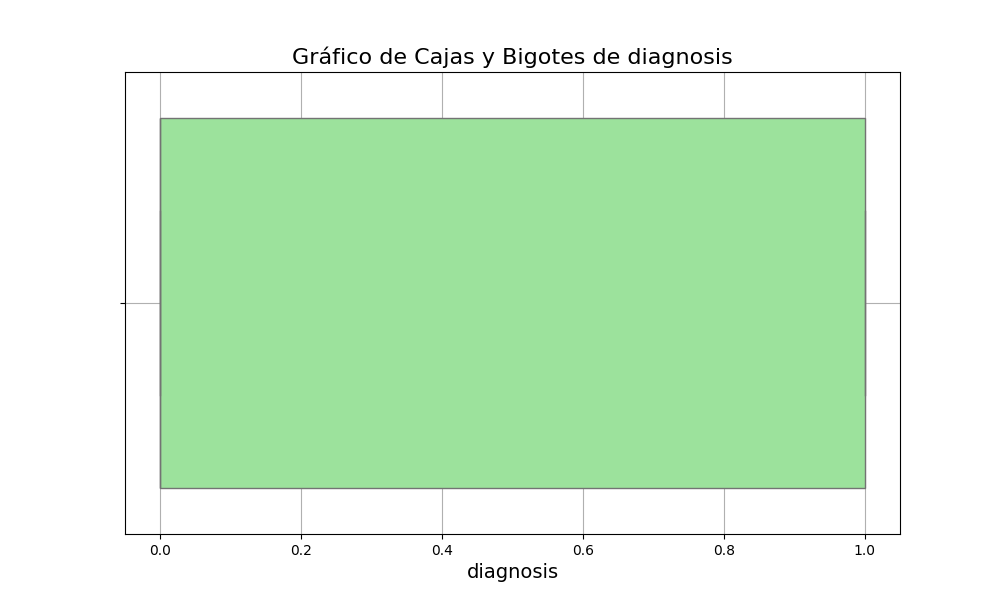
\includegraphics[width=\textwidth]{../Plots/plots_stats/diagnosis/boxplot_diagnosis.png}
	



	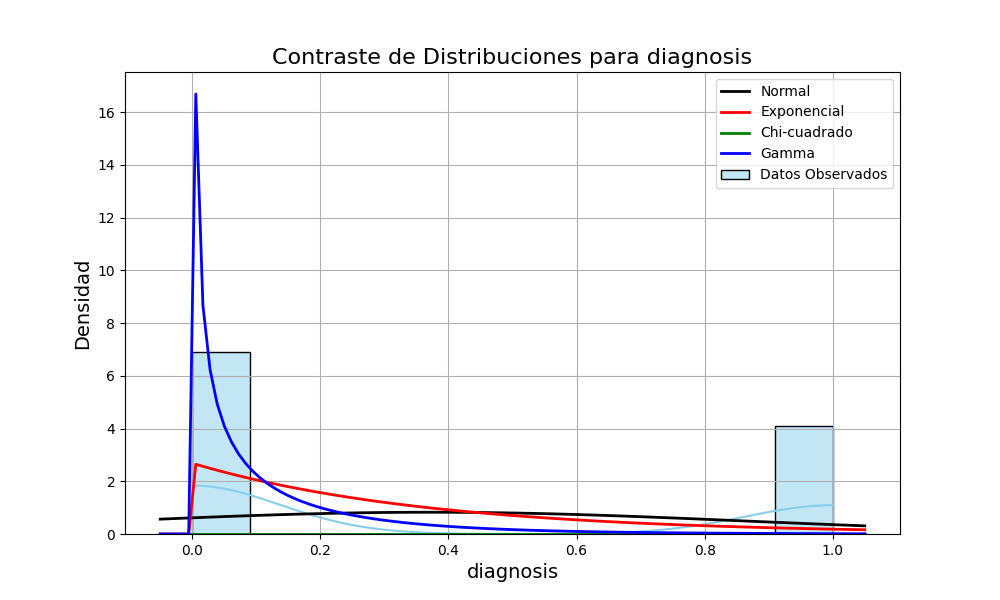
\includegraphics[width=\textwidth]{../Plots/plots_stats/diagnosis/distribuciones_conocidas_diagnosis.png}


\subsection*{\underline{radius\_mean}}

 \begin{itemize}
	\item \textit{Descripción:} Promedio del radio de las células tumorales.
	\item \textit{Medición:} Distancia promedio desde el centro hasta el borde.
	\item \textit{Unidades:} Micrómetros ($\mu$m).
	\item \textit{Interpretación:} Valores más altos indican células más grandes, lo cual puede asociarse con malignidad.
\end{itemize}

	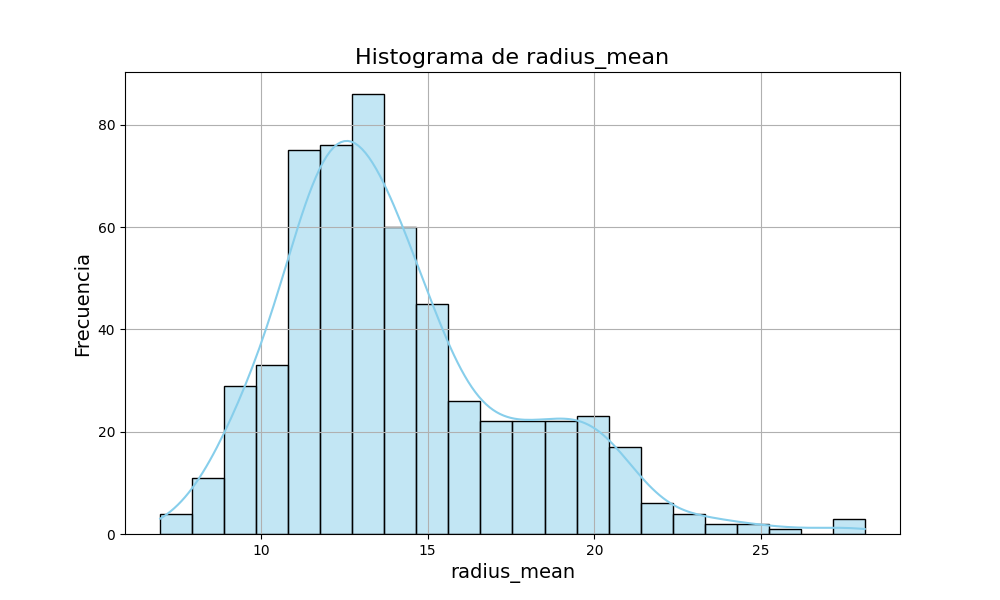
\includegraphics[width=\textwidth]{../Plots/plots_stats/radius_mean/histograma_radius_mean.png}




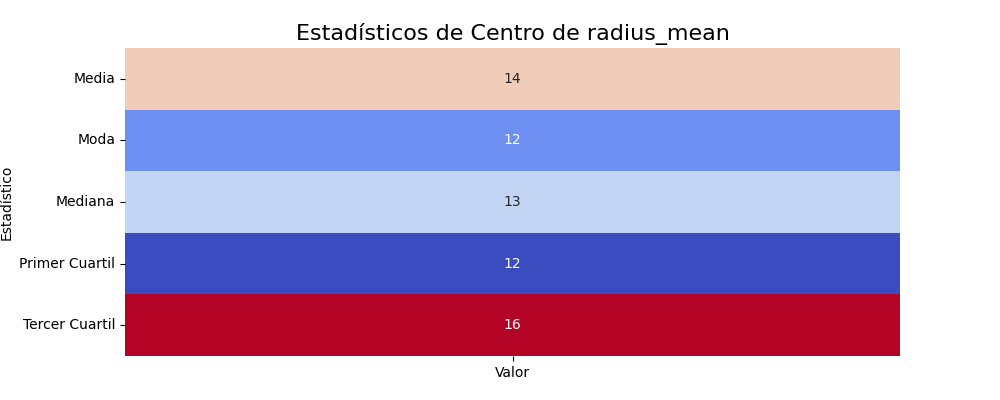
\includegraphics[width=\textwidth]{../Plots/plots_stats/radius_mean/estadisticas_centro_radius_mean.png}




\includegraphics[width=\textwidth]{../Plots/plots_stats/radius_mean/estadisticos_dispersión_radius_mean.png}



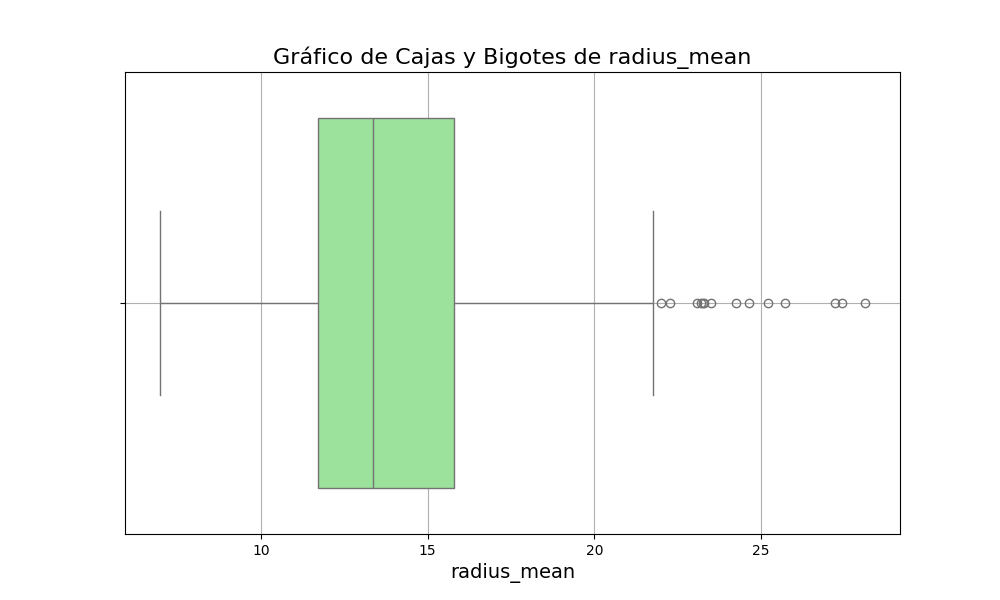
\includegraphics[width=\textwidth]{../Plots/plots_stats/radius_mean/boxplot_radius_mean.png}




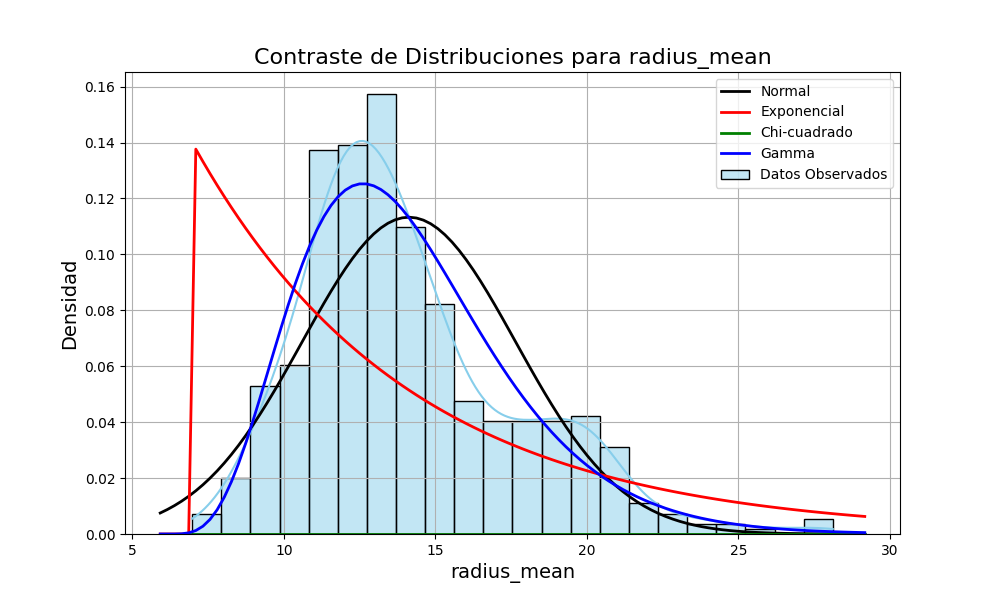
\includegraphics[width=\textwidth]{../Plots/plots_stats/radius_mean/distribuciones_conocidas_radius_mean.png}

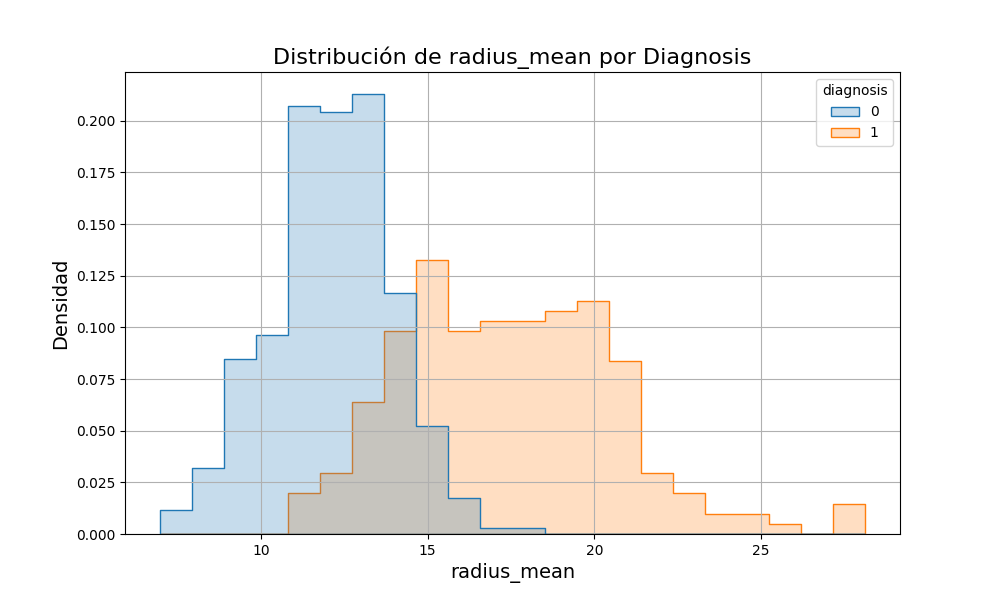
\includegraphics[width=\textwidth]{../Plots/plots_diagnosis/distribucion_radius_mean_por_diagnosis.png}


\subsection*{\underline{texture\_mean}}


    \begin{itemize}
	\item \textit{Descripción:} Promedio de la variación en la intensidad de píxeles.
	\item \textit{Medición:} Promedio de los valores de intensidad.
	\item \textit{Unidades:} Sin unidades (valor adimensional).
	\item \textit{Interpretación:} Valores más altos indican mayor heterogeneidad, lo que sugiere malignidad.
\end{itemize}

	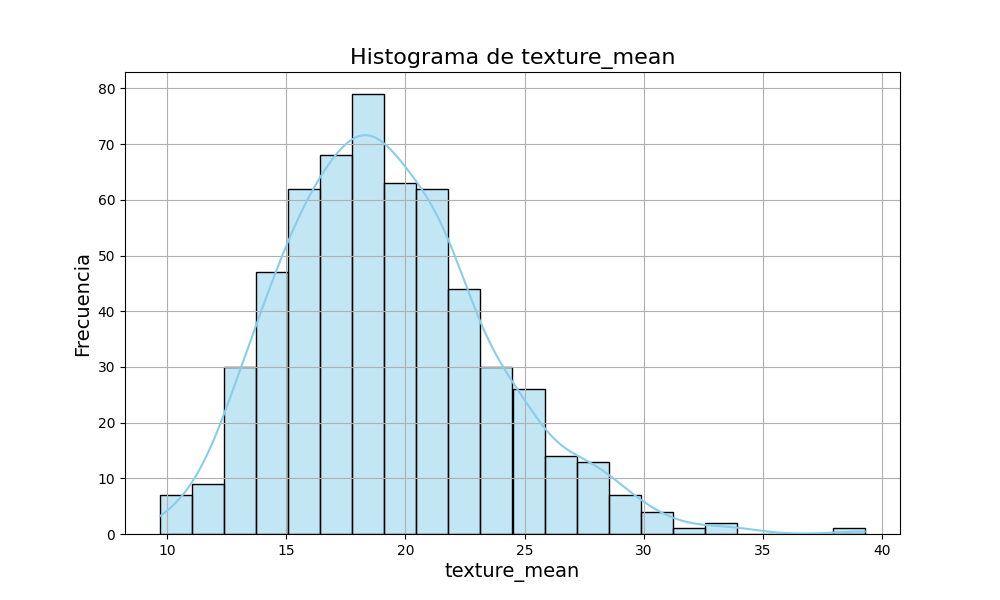
\includegraphics[width=\textwidth]{../Plots/plots_stats/texture_mean/histograma_texture_mean.png}




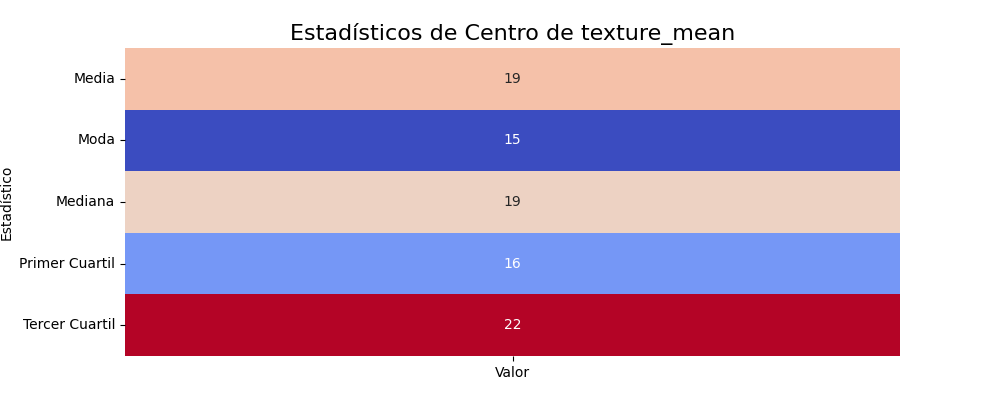
\includegraphics[width=\textwidth]{../Plots/plots_stats/texture_mean/estadisticas_centro_texture_mean.png}




\includegraphics[width=\textwidth]{../Plots/plots_stats/texture_mean/estadisticos_dispersión_texture_mean.png}



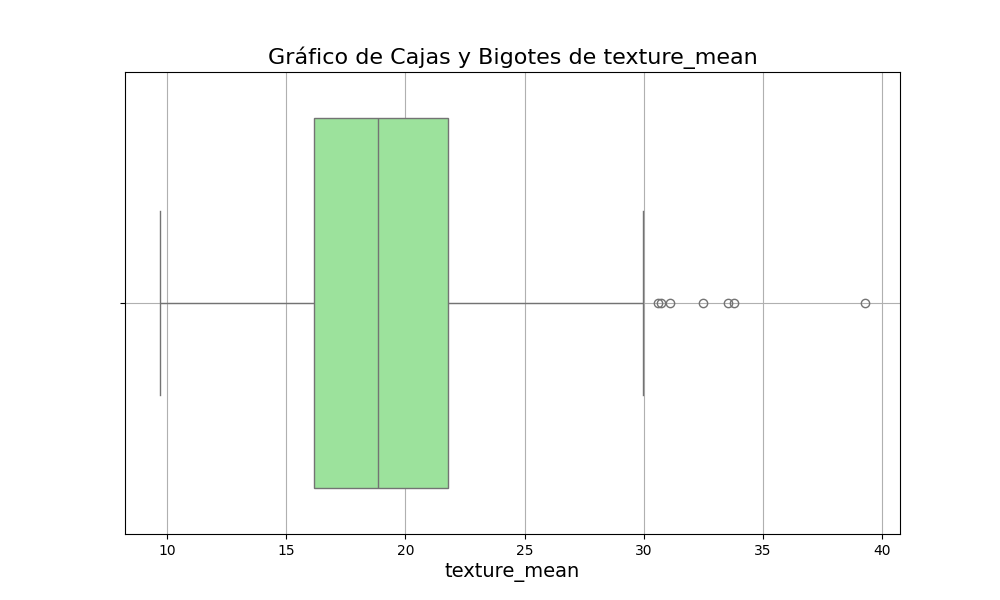
\includegraphics[width=\textwidth]{../Plots/plots_stats/texture_mean/boxplot_texture_mean.png}




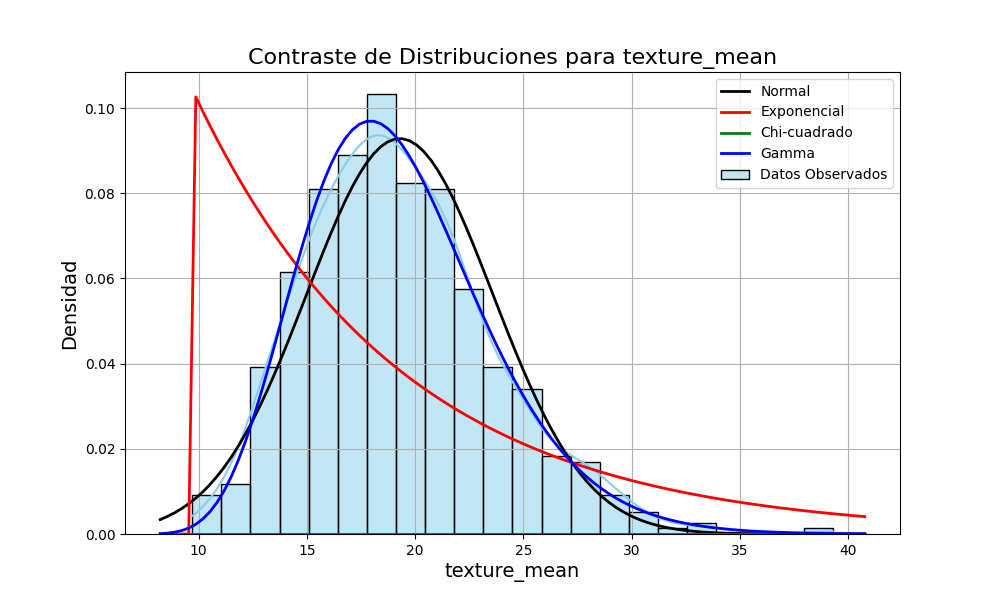
\includegraphics[width=\textwidth]{../Plots/plots_stats/texture_mean/distribuciones_conocidas_texture_mean.png}

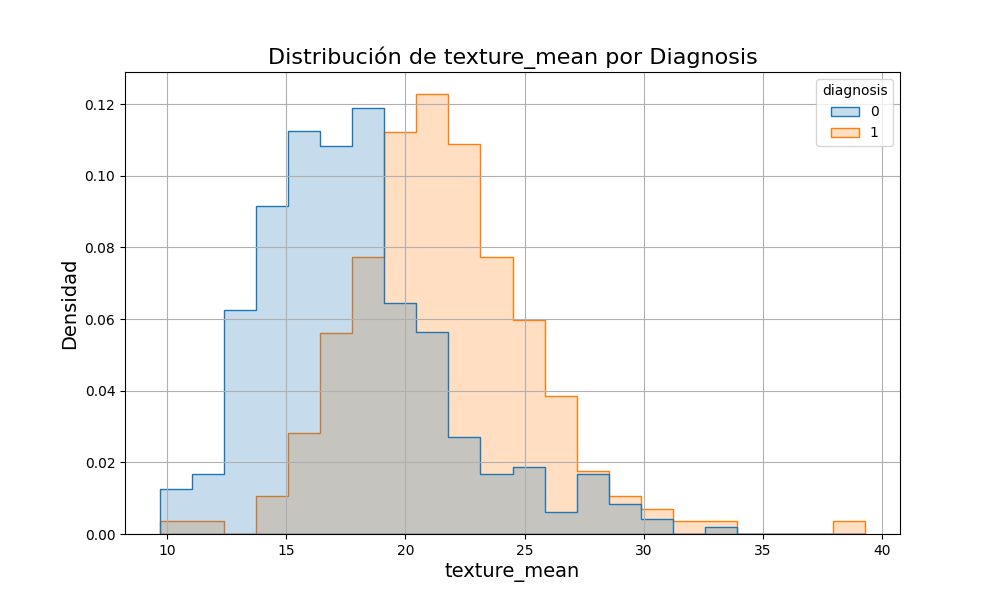
\includegraphics[width=\textwidth]{../Plots/plots_diagnosis/distribucion_texture_mean_por_diagnosis.png}

\subsection*{\underline{perimeter\_mean}}

    \begin{itemize}
	\item \textit{Descripción:} Promedio del perímetro de las células tumorales.
	\item \textit{Medición:} Longitud total de la frontera de la célula.
	\item \textit{Unidades:} Micrómetros ($\mu$m).
\end{itemize}

	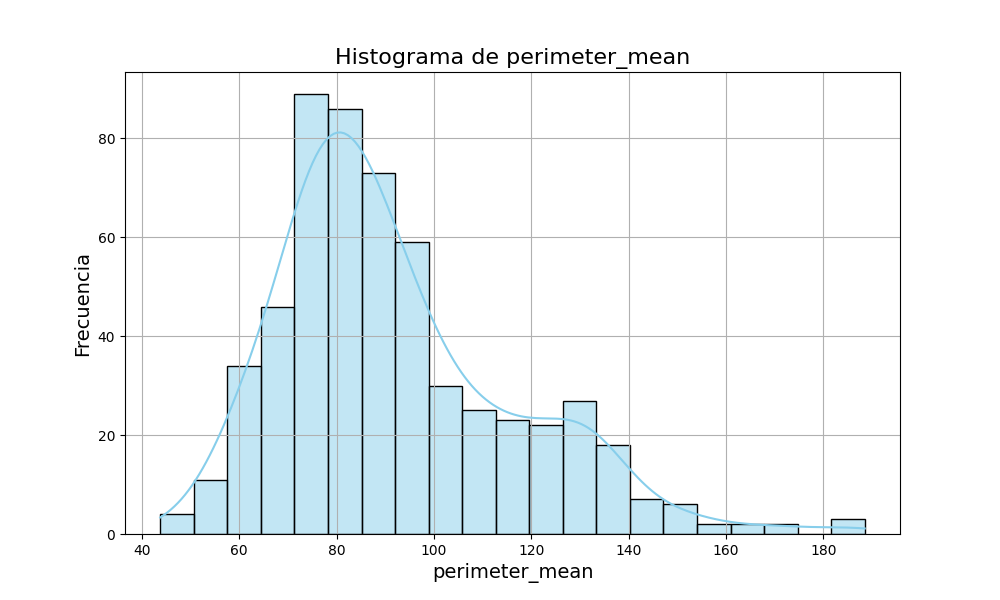
\includegraphics[width=\textwidth]{../Plots/plots_stats/perimeter_mean/histograma_perimeter_mean.png}




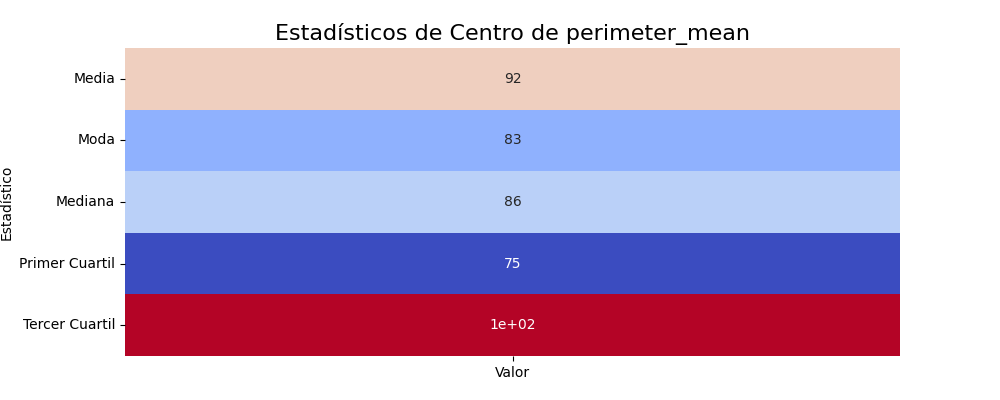
\includegraphics[width=\textwidth]{../Plots/plots_stats/perimeter_mean/estadisticas_centro_perimeter_mean.png}




\includegraphics[width=\textwidth]{../Plots/plots_stats/perimeter_mean/estadisticos_dispersión_perimeter_mean.png}



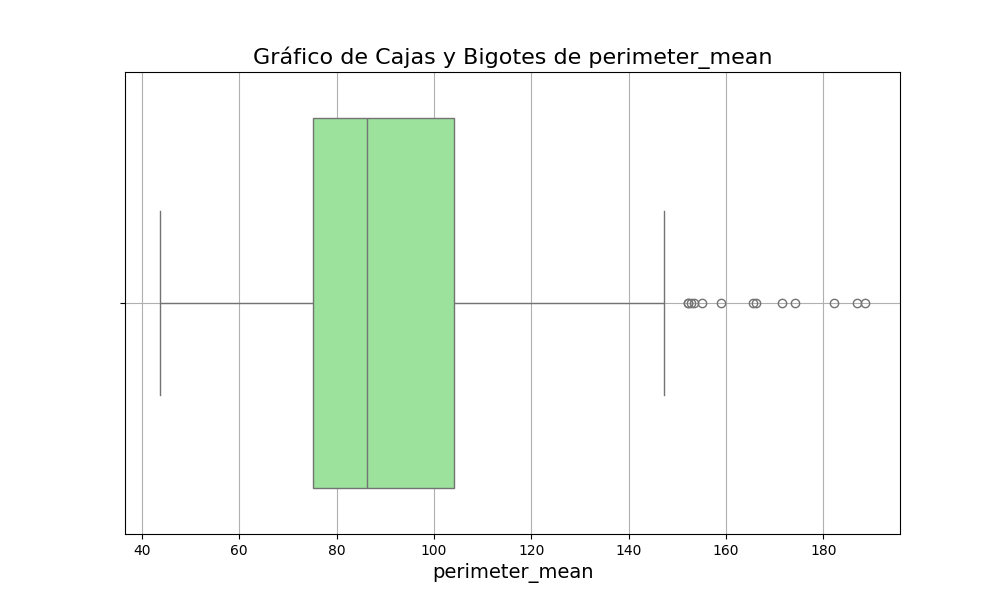
\includegraphics[width=\textwidth]{../Plots/plots_stats/perimeter_mean/boxplot_perimeter_mean.png}




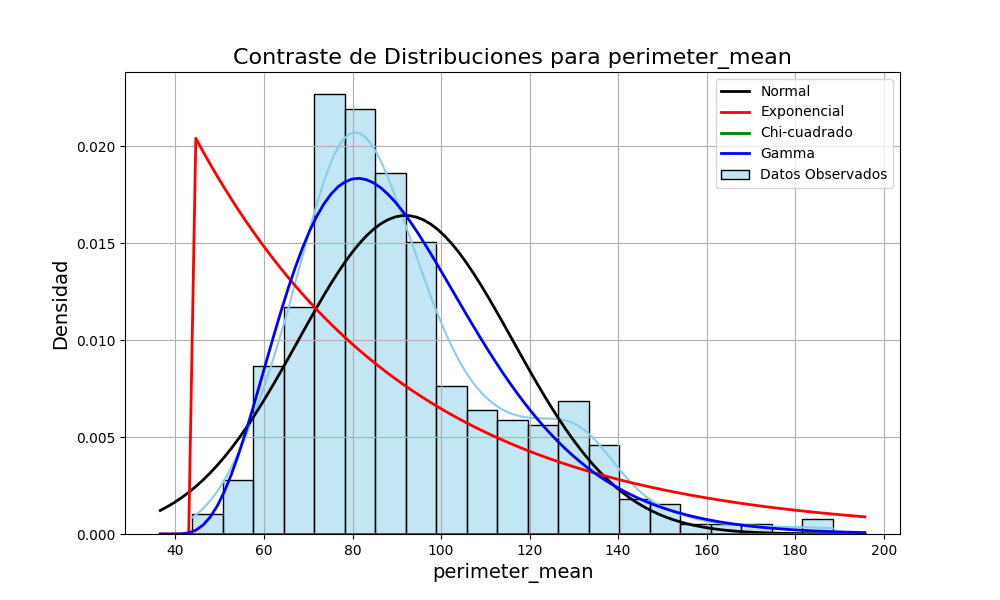
\includegraphics[width=\textwidth]{../Plots/plots_stats/perimeter_mean/distribuciones_conocidas_perimeter_mean.png}

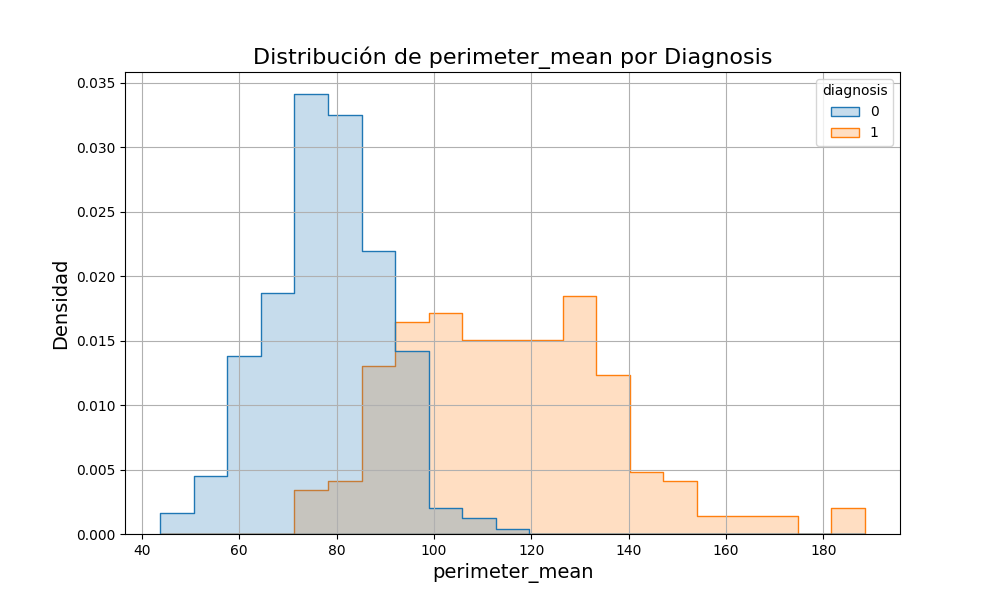
\includegraphics[width=\textwidth]{../Plots/plots_diagnosis/distribucion_perimeter_mean_por_diagnosis.png}


\subsection*{\underline{area\_mean}}

 \begin{itemize}
	\item \textit{Descripción:} Promedio del área de las células tumorales.
	\item \textit{Medición:} Área calculada a partir de la imagen digitalizada.
	\item \textit{Unidades:} Micrómetros cuadrados ($\mu$m$^2$).
\end{itemize}

	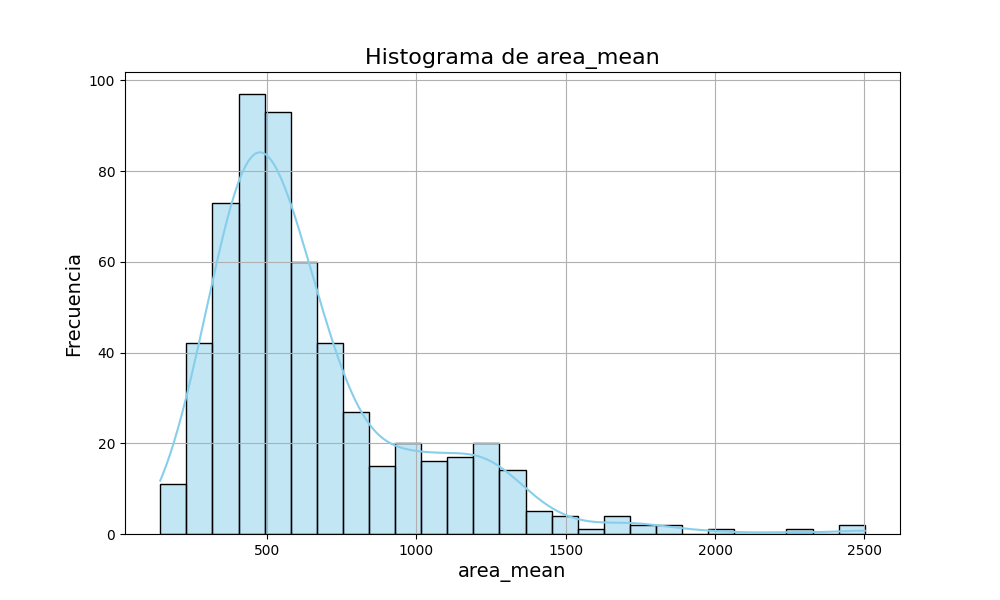
\includegraphics[width=\textwidth]{../Plots/plots_stats/area_mean/histograma_area_mean.png}




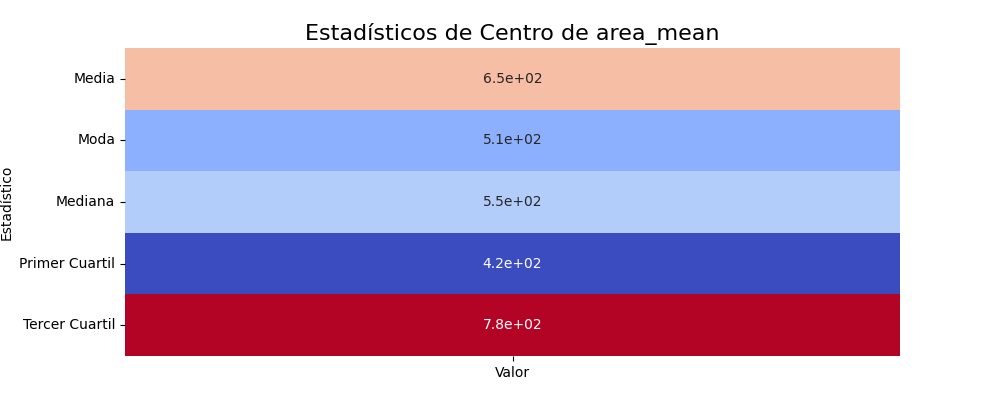
\includegraphics[width=\textwidth]{../Plots/plots_stats/area_mean/estadisticas_centro_area_mean.png}




\includegraphics[width=\textwidth]{../Plots/plots_stats/area_mean/estadisticos_dispersión_area_mean.png}



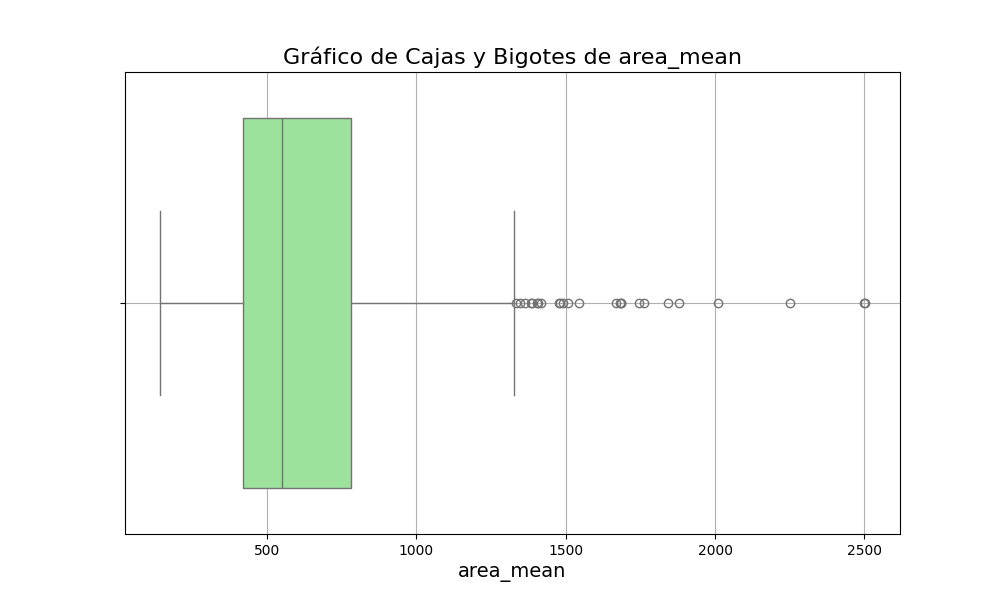
\includegraphics[width=\textwidth]{../Plots/plots_stats/area_mean/boxplot_area_mean.png}




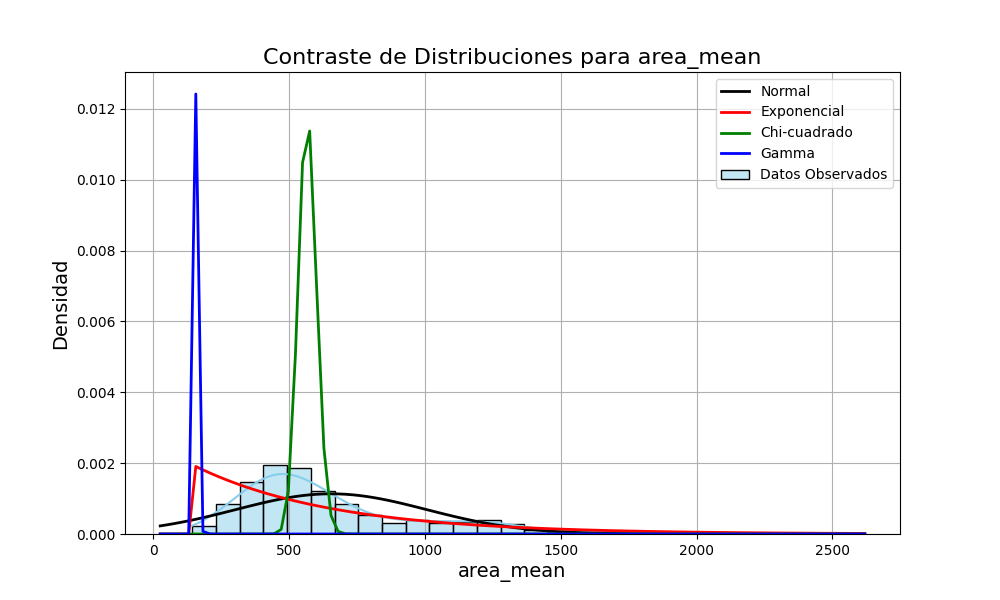
\includegraphics[width=\textwidth]{../Plots/plots_stats/area_mean/distribuciones_conocidas_area_mean.png}

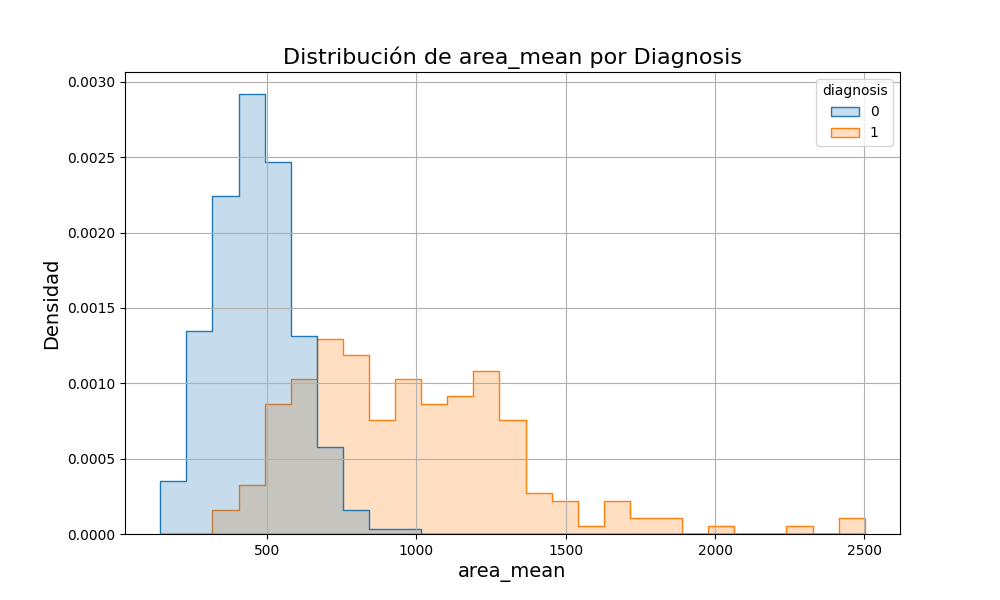
\includegraphics[width=\textwidth]{../Plots/plots_diagnosis/distribucion_area_mean_por_diagnosis.png}

\subsection*{\underline{smoothness\_mean}}

 \begin{itemize}
	\item \textit{Descripción:} Promedio de la uniformidad del contorno de las células.
	\item \textit{Medición:} Variación local de los radios en el contorno.
	\item \textit{Unidades:} Valor adimensional.
\end{itemize}

	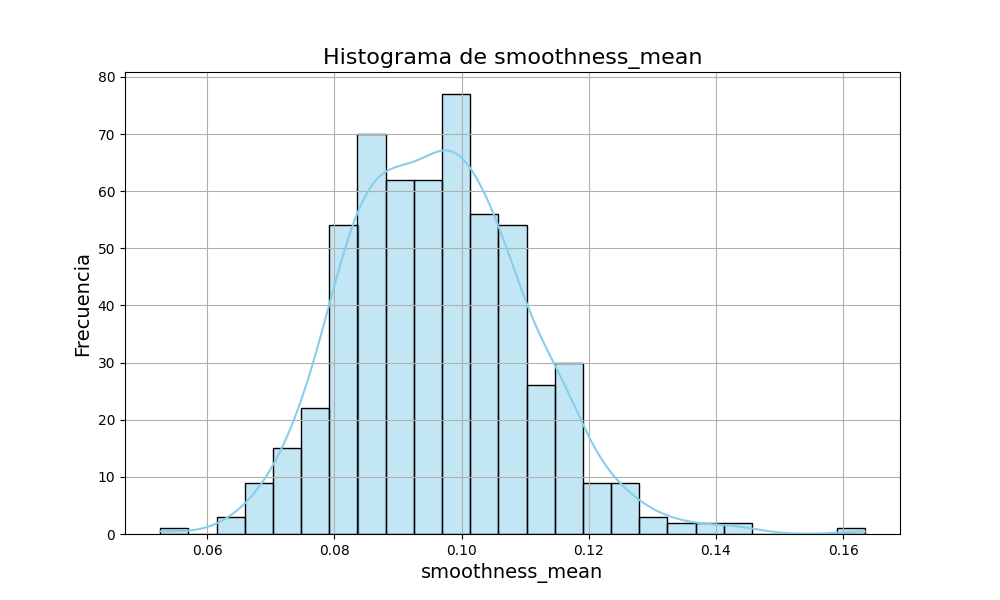
\includegraphics[width=\textwidth]{../Plots/plots_stats/smoothness_mean/histograma_smoothness_mean.png}




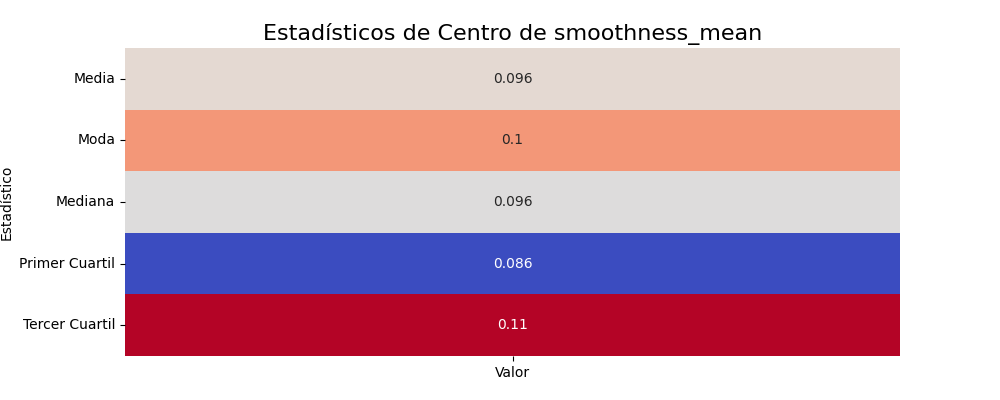
\includegraphics[width=\textwidth]{../Plots/plots_stats/smoothness_mean/estadisticas_centro_smoothness_mean.png}




\includegraphics[width=\textwidth]{../Plots/plots_stats/smoothness_mean/estadisticos_dispersión_smoothness_mean.png}



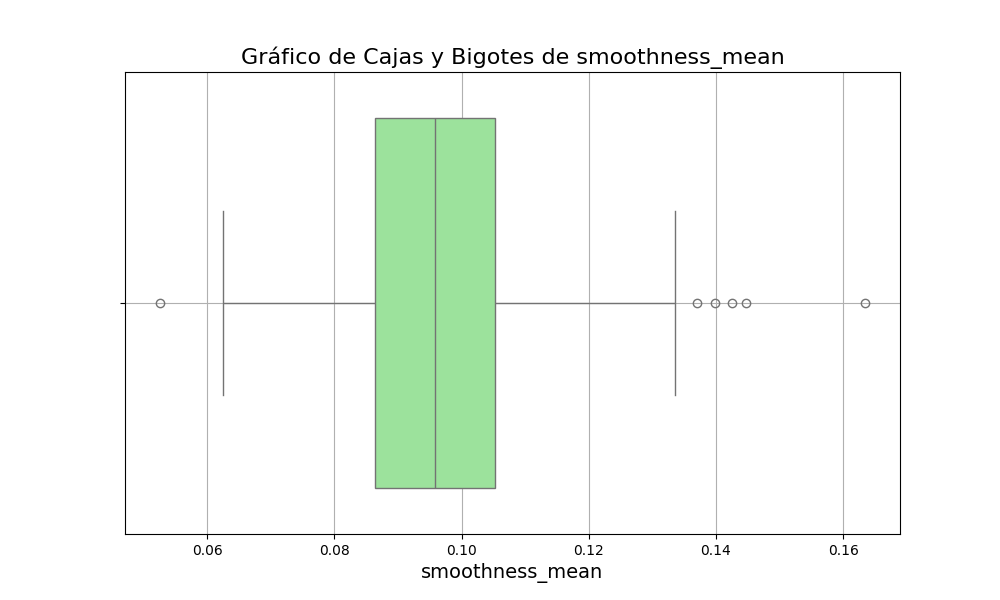
\includegraphics[width=\textwidth]{../Plots/plots_stats/smoothness_mean/boxplot_smoothness_mean.png}




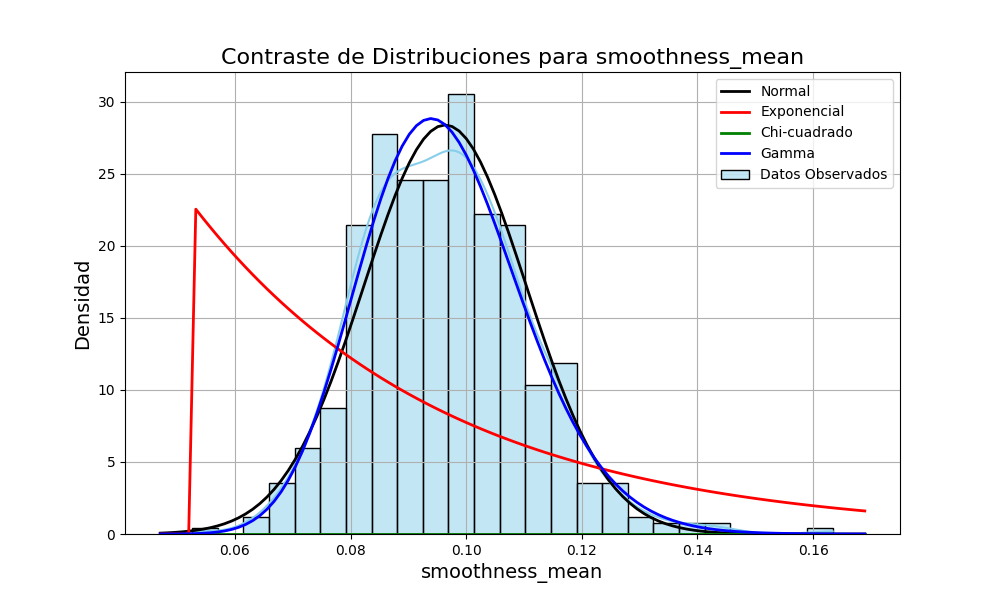
\includegraphics[width=\textwidth]{../Plots/plots_stats/smoothness_mean/distribuciones_conocidas_smoothness_mean.png}

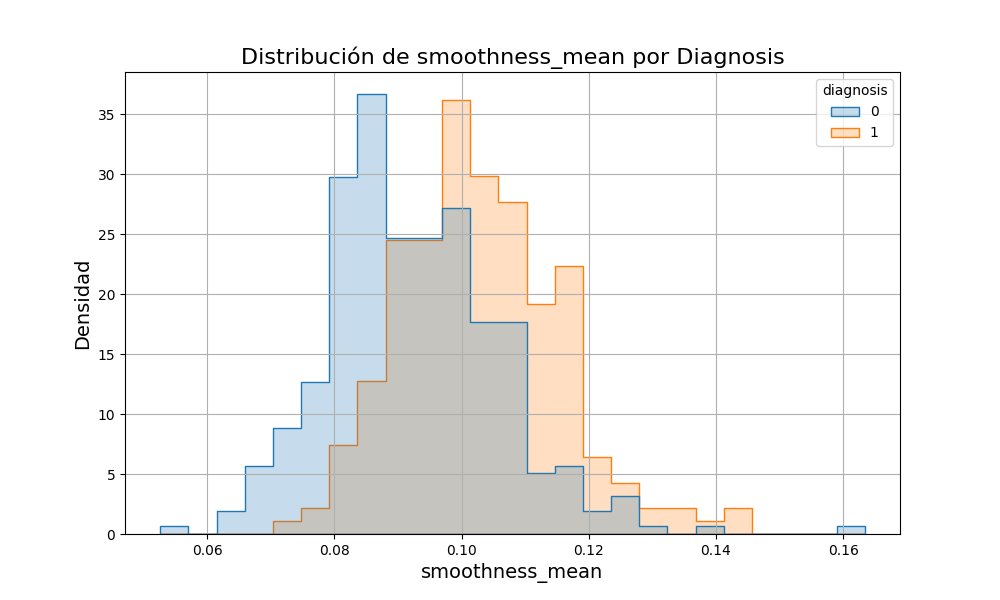
\includegraphics[width=\textwidth]{../Plots/plots_diagnosis/distribucion_smoothness_mean_por_diagnosis.png}

\subsection*{\underline{compactness\_mean}}
  \begin{itemize}
	\item \textit{Descripción:} Promedio de la compacidad de las células.
	\item \textit{Medición:} Relación entre el perímetro y el área:
	\[
	\text{Compactness} = \frac{\text{Perimeter}^2}{\text{Area}} - 1
	\]
	\item \textit{Unidades:} Valor adimensional.
\end{itemize}

	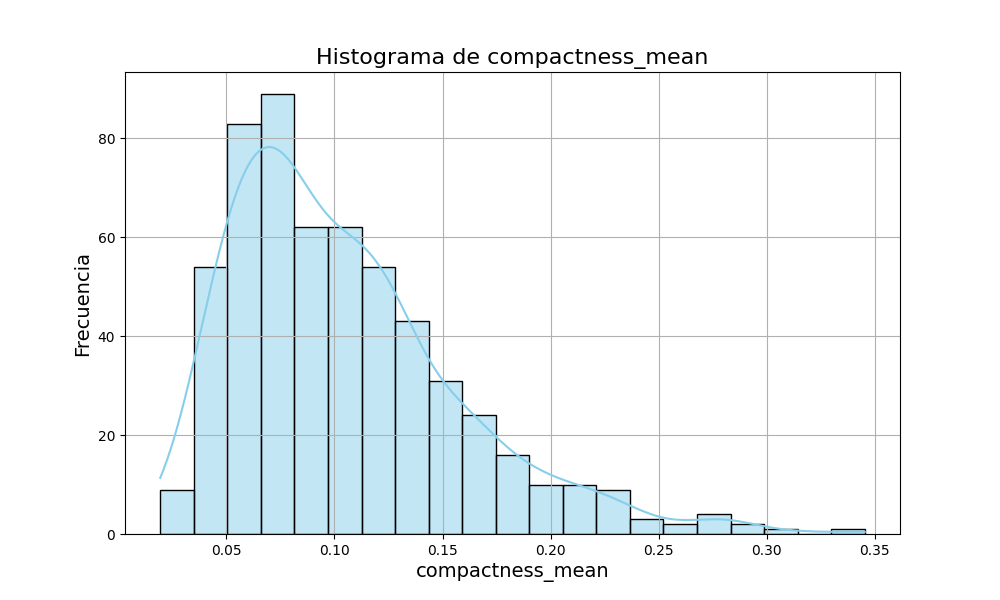
\includegraphics[width=\textwidth]{../Plots/plots_stats/compactness_mean/histograma_compactness_mean.png}




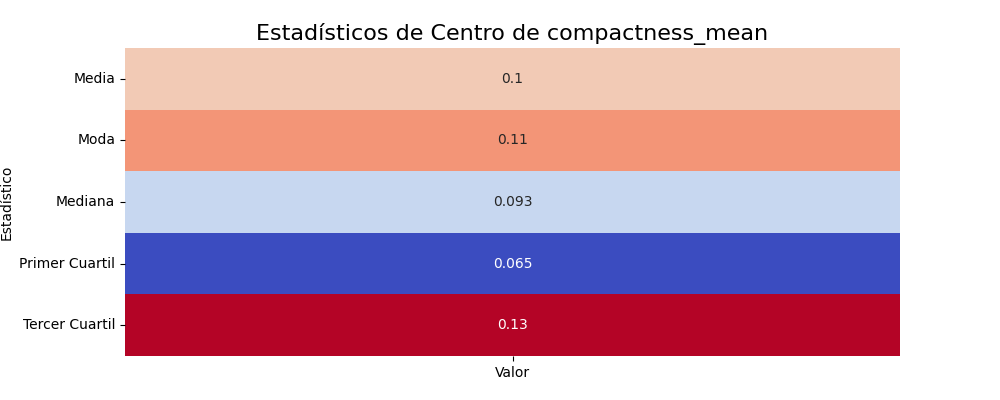
\includegraphics[width=\textwidth]{../Plots/plots_stats/compactness_mean/estadisticas_centro_compactness_mean.png}




\includegraphics[width=\textwidth]{../Plots/plots_stats/compactness_mean/estadisticos_dispersión_compactness_mean.png}



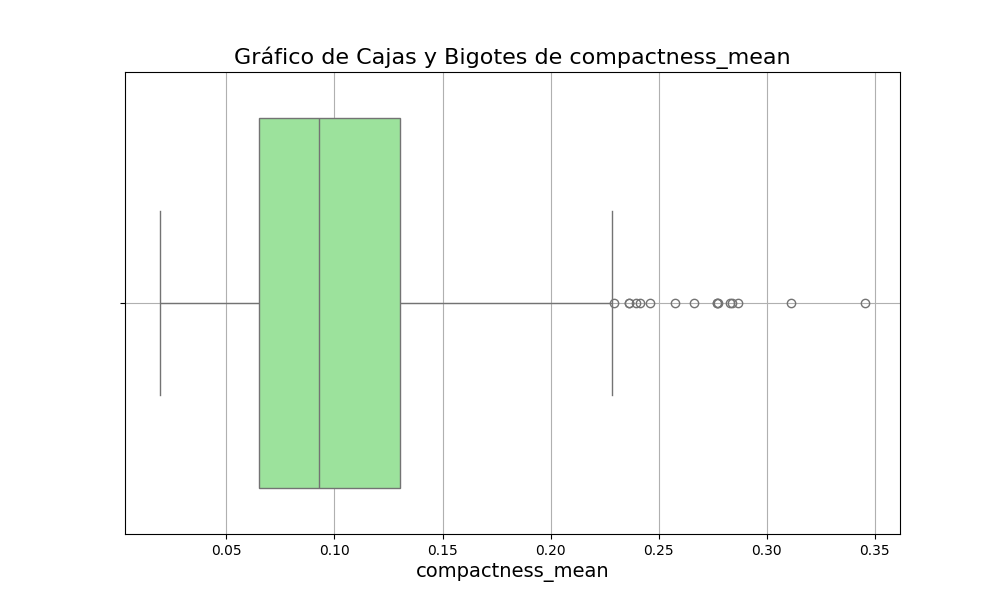
\includegraphics[width=\textwidth]{../Plots/plots_stats/compactness_mean/boxplot_compactness_mean.png}




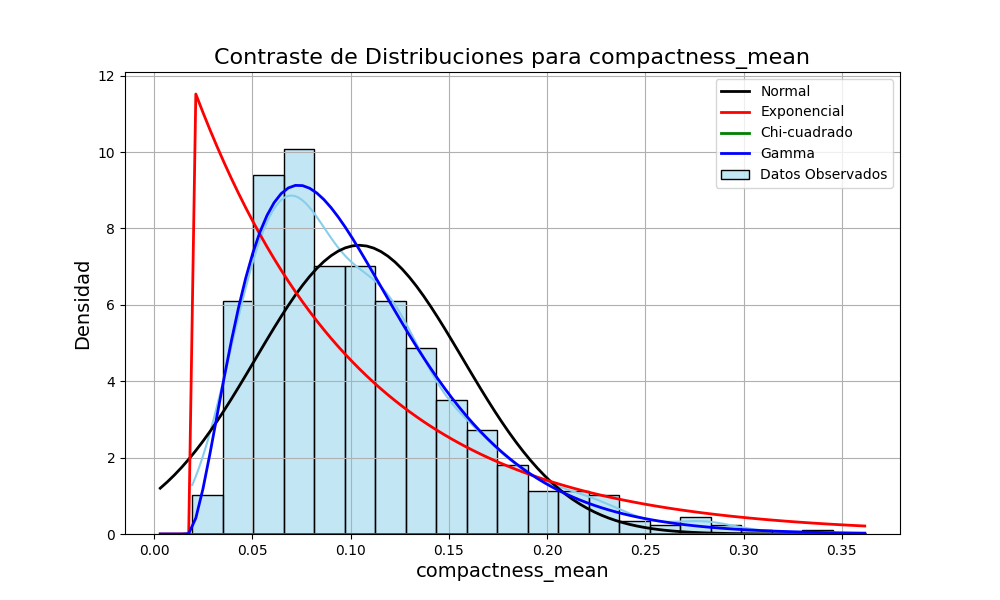
\includegraphics[width=\textwidth]{../Plots/plots_stats/compactness_mean/distribuciones_conocidas_compactness_mean.png}

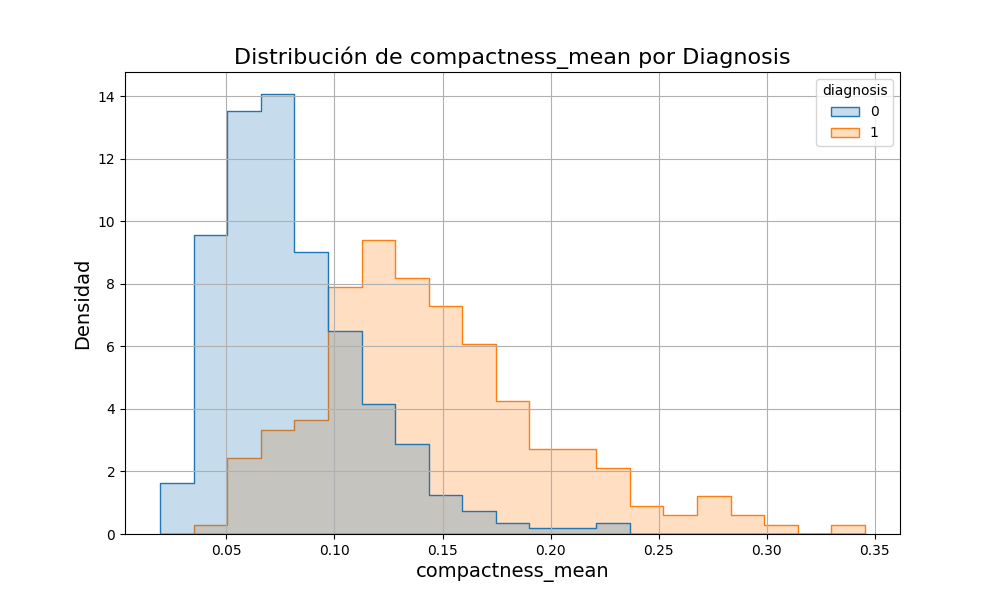
\includegraphics[width=\textwidth]{../Plots/plots_diagnosis/distribucion_compactness_mean_por_diagnosis.png}

\subsection*{\underline{symmetry\_mean}}
    \begin{itemize}
	\item \textit{Descripción:} Promedio de la simetría de las células.
	\item \textit{Medición:} Diferencia entre los radios en distintas direcciones.
	\item \textit{Unidades:} Valor adimensional.
\end{itemize}

	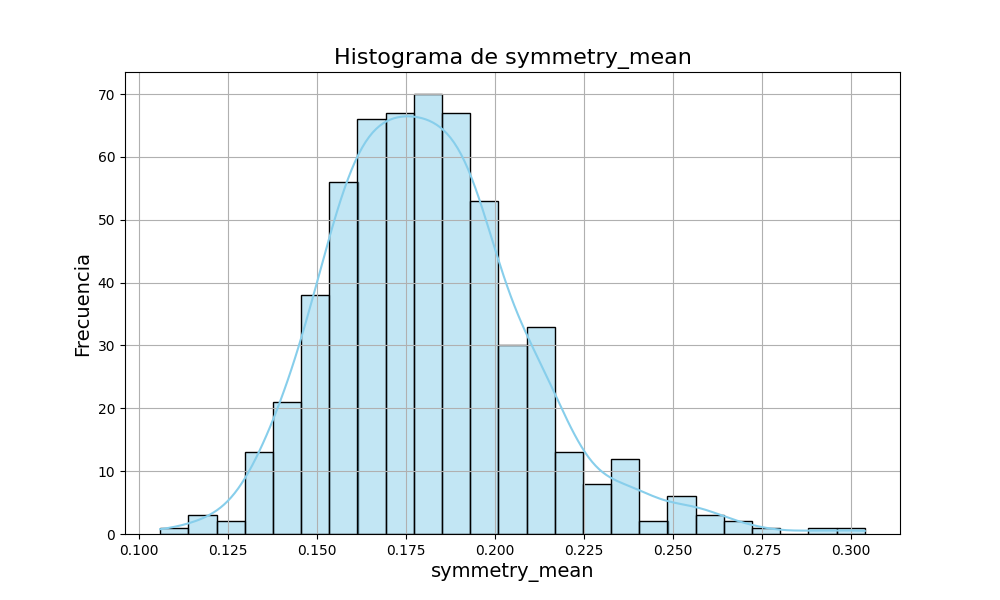
\includegraphics[width=\textwidth]{../Plots/plots_stats/symmetry_mean/histograma_symmetry_mean.png}




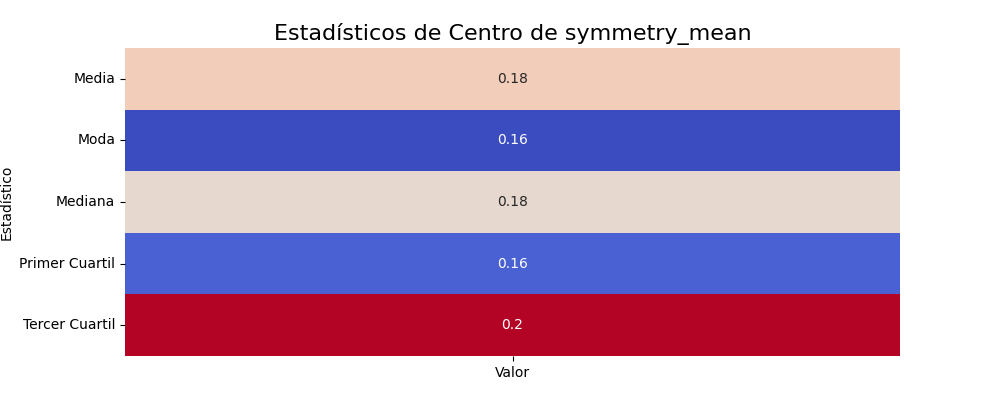
\includegraphics[width=\textwidth]{../Plots/plots_stats/symmetry_mean/estadisticas_centro_symmetry_mean.png}




\includegraphics[width=\textwidth]{../Plots/plots_stats/symmetry_mean/estadisticos_dispersión_symmetry_mean.png}



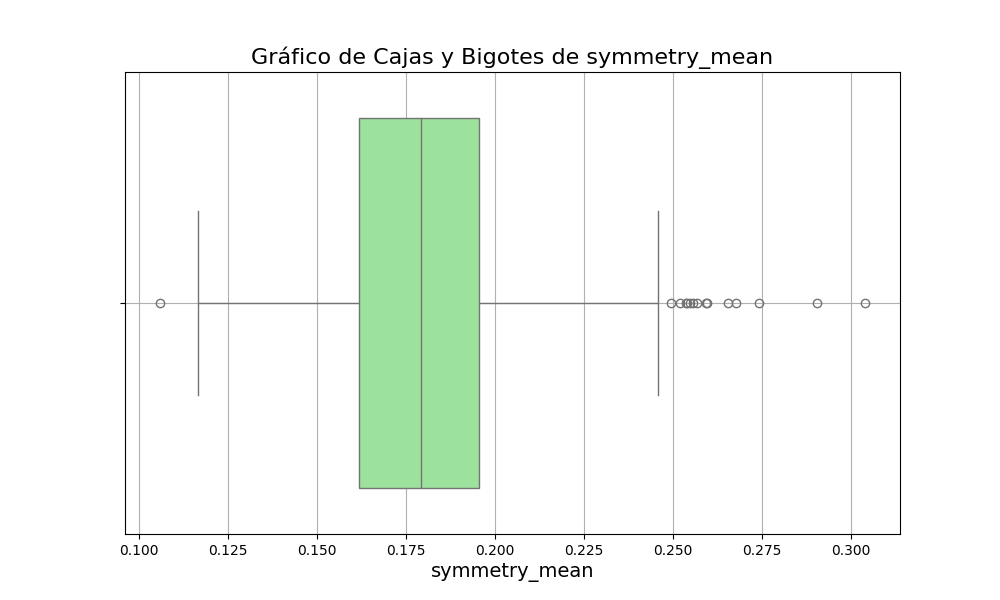
\includegraphics[width=\textwidth]{../Plots/plots_stats/symmetry_mean/boxplot_symmetry_mean.png}




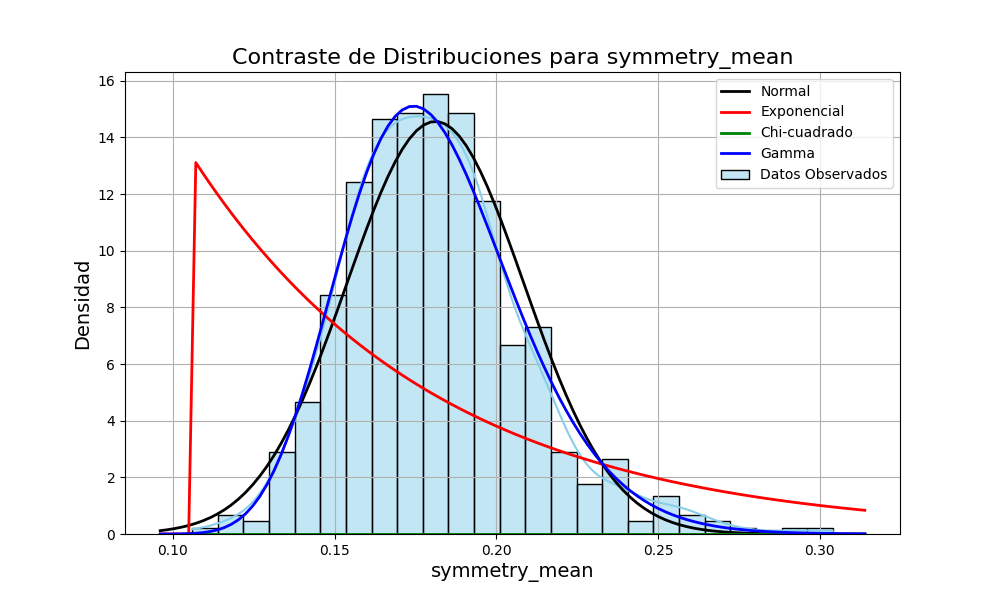
\includegraphics[width=\textwidth]{../Plots/plots_stats/symmetry_mean/distribuciones_conocidas_symmetry_mean.png}

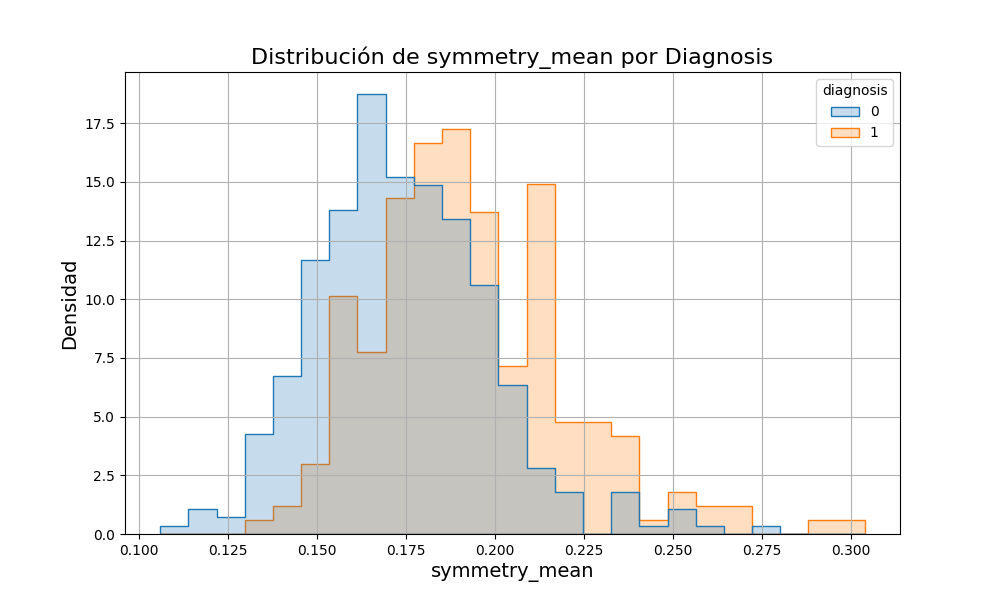
\includegraphics[width=\textwidth]{../Plots/plots_diagnosis/distribucion_symmetry_mean_por_diagnosis.png}

\newpage 

\textbf{radius\_worst, texture\_worst, perimeter\_worst, area\_worst, smoothness\_worst, compactness\_worst, symmetry\_worst}:
\begin{itemize}
	\item \textit{Descripción:} Estas variables representan los valores extremos (peores) observados en la medición de las características anteriores.
	\item \textit{Medición:} Se calculan de la misma manera que las variables \_mean pero enfocándose en los valores máximos registrados.
\end{itemize}



\subsection*{\underline{radius\_worst}}

	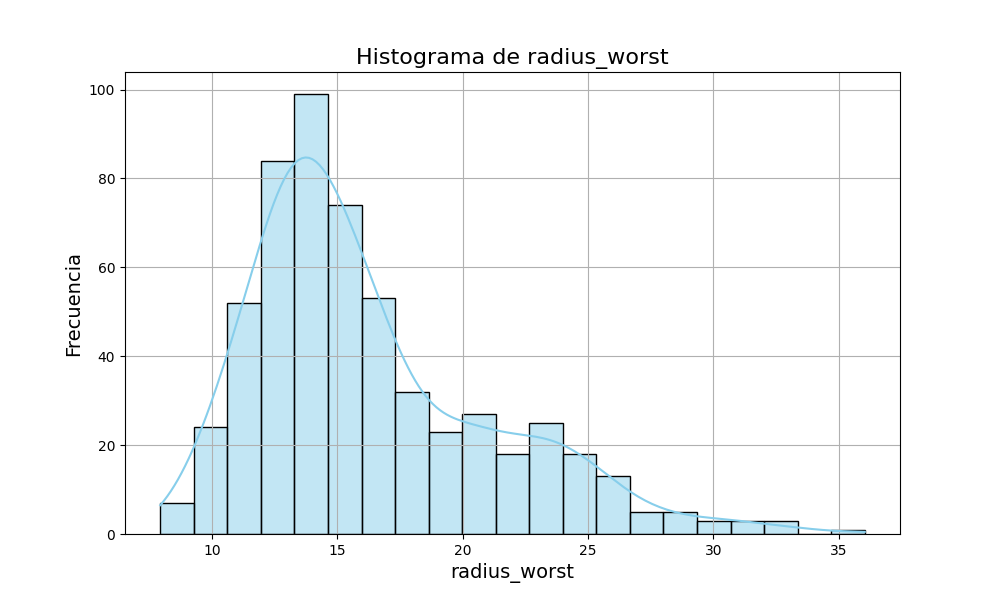
\includegraphics[width=\textwidth]{../Plots/plots_stats/radius_worst/histograma_radius_worst.png}




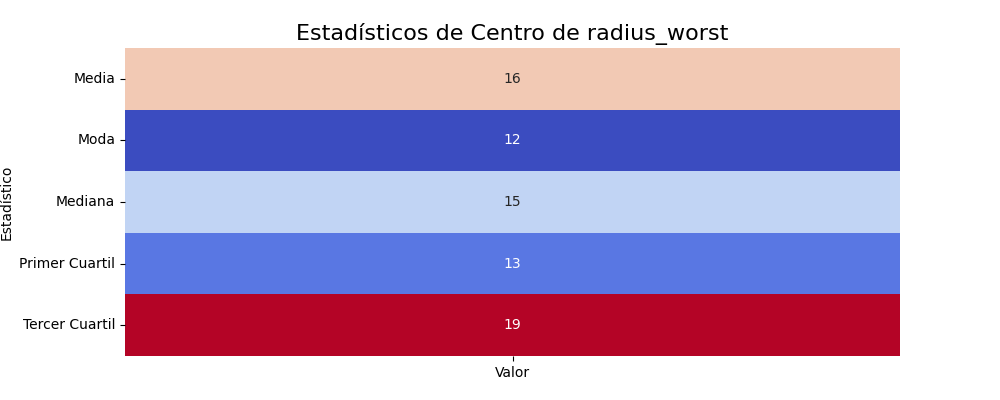
\includegraphics[width=\textwidth]{../Plots/plots_stats/radius_worst/estadisticas_centro_radius_worst.png}




\includegraphics[width=\textwidth]{../Plots/plots_stats/radius_worst/estadisticos_dispersión_radius_worst.png}



\includegraphics[width=\textwidth]{../Plots/plots_stats/radius_worst/boxplot_radius_worst.png}




\includegraphics[width=\textwidth]{../Plots/plots_stats/radius_worst/distribuciones_conocidas_radius_worst.png}

\includegraphics[width=\textwidth]{../Plots/plots_diagnosis/distribucion_radius_worst_por_diagnosis.png}


\subsection*{\underline{texture\_worst}}

	\includegraphics[width=\textwidth]{../Plots/plots_stats/texture_worst/histograma_texture_worst.png}




\includegraphics[width=\textwidth]{../Plots/plots_stats/texture_worst/estadisticas_centro_texture_worst.png}




\includegraphics[width=\textwidth]{../Plots/plots_stats/texture_worst/estadisticos_dispersión_texture_worst.png}



\includegraphics[width=\textwidth]{../Plots/plots_stats/texture_worst/boxplot_texture_worst.png}




\includegraphics[width=\textwidth]{../Plots/plots_stats/texture_worst/distribuciones_conocidas_texture_worst.png}

\includegraphics[width=\textwidth]{../Plots/plots_diagnosis/distribucion_texture_worst_por_diagnosis.png}

\subsection*{\underline{perimeter\_worst}}

	\includegraphics[width=\textwidth]{../Plots/plots_stats/perimeter_worst/histograma_perimeter_worst.png}




\includegraphics[width=\textwidth]{../Plots/plots_stats/perimeter_worst/estadisticas_centro_perimeter_worst.png}




\includegraphics[width=\textwidth]{../Plots/plots_stats/perimeter_worst/estadisticos_dispersión_perimeter_worst.png}



\includegraphics[width=\textwidth]{../Plots/plots_stats/perimeter_worst/boxplot_perimeter_worst.png}




\includegraphics[width=\textwidth]{../Plots/plots_stats/perimeter_worst/distribuciones_conocidas_perimeter_worst.png}

\includegraphics[width=\textwidth]{../Plots/plots_diagnosis/distribucion_perimeter_worst_por_diagnosis.png}

\subsection*{\underline{area\_worst}}

	\includegraphics[width=\textwidth]{../Plots/plots_stats/area_worst/histograma_area_worst.png}




\includegraphics[width=\textwidth]{../Plots/plots_stats/area_worst/estadisticas_centro_area_worst.png}




\includegraphics[width=\textwidth]{../Plots/plots_stats/area_worst/estadisticos_dispersión_area_worst.png}



\includegraphics[width=\textwidth]{../Plots/plots_stats/area_worst/boxplot_area_worst.png}




\includegraphics[width=\textwidth]{../Plots/plots_stats/area_worst/distribuciones_conocidas_area_worst.png}

\includegraphics[width=\textwidth]{../Plots/plots_diagnosis/distribucion_area_worst_por_diagnosis.png}

\subsection*{\underline{smoothness\_worst}}

	\includegraphics[width=\textwidth]{../Plots/plots_stats/smoothness_worst/histograma_smoothness_worst.png}




\includegraphics[width=\textwidth]{../Plots/plots_stats/smoothness_worst/estadisticas_centro_smoothness_worst.png}




\includegraphics[width=\textwidth]{../Plots/plots_stats/smoothness_worst/estadisticos_dispersión_smoothness_worst.png}



\includegraphics[width=\textwidth]{../Plots/plots_stats/smoothness_worst/boxplot_smoothness_worst.png}




\includegraphics[width=\textwidth]{../Plots/plots_stats/smoothness_worst/distribuciones_conocidas_smoothness_worst.png}

\includegraphics[width=\textwidth]{../Plots/plots_diagnosis/distribucion_smoothness_worst_por_diagnosis.png}

\subsection*{\underline{compactness\_worst}}

	\includegraphics[width=\textwidth]{../Plots/plots_stats/smoothness_worst/histograma_smoothness_worst.png}




\includegraphics[width=\textwidth]{../Plots/plots_stats/smoothness_worst/estadisticas_centro_smoothness_worst.png}




\includegraphics[width=\textwidth]{../Plots/plots_stats/smoothness_worst/estadisticos_dispersión_smoothness_worst.png}



\includegraphics[width=\textwidth]{../Plots/plots_stats/smoothness_worst/boxplot_smoothness_worst.png}




\includegraphics[width=\textwidth]{../Plots/plots_stats/smoothness_worst/distribuciones_conocidas_smoothness_worst.png}

\includegraphics[width=\textwidth]{../Plots/plots_diagnosis/distribucion_smoothness_worst_por_diagnosis.png}

\subsection*{\underline{symmetry\_worst}}

	\includegraphics[width=\textwidth]{../Plots/plots_stats/symmetry_worst/histograma_symmetry_worst.png}




\includegraphics[width=\textwidth]{../Plots/plots_stats/symmetry_worst/estadisticas_centro_symmetry_worst.png}




\includegraphics[width=\textwidth]{../Plots/plots_stats/symmetry_worst/estadisticos_dispersión_symmetry_worst.png}



\includegraphics[width=\textwidth]{../Plots/plots_stats/symmetry_worst/boxplot_symmetry_worst.png}




\includegraphics[width=\textwidth]{../Plots/plots_stats/symmetry_worst/distribuciones_conocidas_symmetry_worst.png}

\includegraphics[width=\textwidth]{../Plots/plots_diagnosis/distribucion_symmetry_worst_por_diagnosis.png}


\newpage

\section{Análisis de la distribución}

\subsection{Pruebas de Normalidad}

\subsection*{Kolmogorov-Smirnov}
\includegraphics[width=\textwidth]{../Plots/resumen_normalidad.png}

\subsection*{Shapiro-Wilk}
\includegraphics[width=\textwidth]{../Plots/resumen_shapiro_wilk.png}

\subsection*{Anderson-Darling}
\includegraphics[width=\textwidth]{../Plots/resumen_anderson_darling.png}


\subsection{Estimación de parámetros}

\subsubsection{texture\_mean}

\textbf{Estimación Puntual}

\textbf{Estimación por Intervalos}


\subsubsection{smoothness\_mean}

\textbf{Estimación Puntual}

\textbf{Estimación por Intervalos}


\subsubsection{symmetry\_mean}

\textbf{Estimación Puntual}

\textbf{Estimación por Intervalos}


\subsubsection{texture\_worst}

\textbf{Estimación Puntual}

\textbf{Estimación por Intervalos}


\subsubsection{smoothness\_worst}

\textbf{Estimación Puntual}

\textbf{Estimación por Intervalos}


\subsubsection{diagnosis}

\textbf{Estimación Puntual}

\textbf{Estimación por Intervalos}


\subsection{Pruebas de Hipótesis}

\subsubsection{Pruebas de Hipótesis para una población}

\textbf{Ejemplo 1: Media de una población conocida}\\

Se desea verificar si la media de la variable \textit{texture\_mean} es igual a 20. 

\begin{itemize}
	\item \textbf{Hipótesis nula} (\(H_0\)): \(\mu = 20\)
	\item \textbf{Hipótesis alternativa} (\(H_a\)): \(\mu \neq 20\)
\end{itemize}

\textbf{Prueba}: Estadístico \( Z = \frac{\bar{x} - \mu}{\sigma / \sqrt{n}} \)\\

\textbf{Ejemplo 2: Proporción de una población}\\

Se desea verificar si la proporción de diagnósticos de tipo \textit{Maligno} es mayor al 50\%.

\begin{itemize}
	\item \textbf{Hipótesis nula} (\(H_0\)): \(p = 0.5\)
	\item \textbf{Hipótesis alternativa} (\(H_a\)): \(p > 0.5\)
\end{itemize}

\textbf{Prueba}: Estadístico \( Z = \frac{\hat{p} - p}{\sqrt{\frac{p(1-p)}{n}}} \)\\

\textbf{Ejemplo 3: Varianza de una población}\\

Se desea verificar si la varianza de la variable \textit{symmetry\_mean} es igual a 0.001. 

\begin{itemize}
	\item \textbf{Hipótesis nula} (\(H_0\)): \(\sigma^2 = 0.001\)
	\item \textbf{Hipótesis alternativa} (\(H_a\)): \(\sigma^2 \neq 0.001\)
\end{itemize}

\textbf{Prueba}: Estadístico \(\chi^2 = \frac{(n-1)S^2}{\sigma^2}\)\\
\textbf{Ejemplo 4: Media de una población con varianza desconocida}\\

Se desea verificar si la media de la variable \textit{texture\_worst} es mayor a 20.(Varianza desconocida)

\begin{itemize}
	\item \textbf{Hipótesis nula} (\(H_0\)): \(\mu \leq 20\)
	\item \textbf{Hipótesis alternativa} (\(H_a\)): \(\mu > 20\)
\end{itemize}

\textbf{Prueba}: Estadístico \( t = \frac{\bar{x} - \mu}{\sigma / \sqrt{n}} \)\\

\subsubsection{Pruebas de Hipótesis para dos poblaciones}

\textbf{Ejemplo 1: Igualdad de medias}

Se desea verificar si la media de la variable \textit{smoothness\_worst} es igual en los grupos \textit{Maligno} y \textit{Benigno}.(Varianzas Desconocidas).
Primero efectuar prueba para saber si son iguales o diferentes.

\begin{itemize}
	\item \textbf{Hipótesis nula} (\(H_0\)): \(\mu_1 = \mu_2\)
	\item \textbf{Hipótesis alternativa} (\(H_a\)): \(\mu_1 \neq \mu_2\)
\end{itemize}

\textbf{Prueba}: \(t = \frac{(\bar{x}_1 - \bar{x}_2)}{\sqrt{s_1^2/n_1 + s_2^2/n_2}}\)\\

\textbf{Ejemplo 2: Igualdad de proporciones}\\

Se desea verificar si la proporción de diagnósticos malignos es diferente entre dos grupos(a decidir todavía).

\begin{itemize}
	\item \textbf{Hipótesis nula} (\(H_0\)): \(p_1 = p_2\)
	\item \textbf{Hipótesis alternativa} (\(H_a\)): \(p_1 \neq p_2\)
\end{itemize}

\textbf{Prueba}: \(Z = \frac{(\hat{p}_1 - \hat{p}_2)}{\sqrt{\hat{p}(1-\hat{p})(1/n_1 + 1/n_2)}}\), donde \(\hat{p}\) es la proporción conjunta.\\

\textbf{Ejemplo 3: Igualdad de varianzas}\\

Se desea verificar si la varianza de la variable \textit{symmetry\_mean} es igual en los grupos \textit{Maligno} y \textit{Benigno}.

\begin{itemize}
	\item \textbf{Hipótesis nula} (\(H_0\)): \(\sigma_1^2 = \sigma_2^2\)
	\item \textbf{Hipótesis alternativa} (\(H_a\)): \(\sigma_1^2 \neq \sigma_2^2\)
\end{itemize}

\textbf{Prueba}: \(F = \frac{s_1^2}{s_2^2}\)


\newpage

\section{Correlación e Independencia}
\subsection{Correlación}
	\includegraphics[width = \textwidth]{../Plots/plots_corr/corr_matrix/matriz_correlacion_pearson.png}



	\includegraphics[width = \textwidth]{../Plots/plots_corr/corr_matrix/matriz_correlacion_spearman.png}

	De acuerdo a los resultados obtenidos se realizará un análisis más detallado de las variables con mayor correlación.

\subsubsection{area\_mean\_vs\_area\_worst}
	\includegraphics[width = \textwidth]{../Plots/plots_corr/area_mean_vs_area_worst/coeficiente_correlacion_area_mean_vs_area_worst.png}
	\includegraphics[width = \textwidth]{../Plots/plots_corr/area_mean_vs_area_worst/dispersión_area_mean_vs_area_worst.png}
	\includegraphics[width = \textwidth]{../Plots/plots_corr/area_mean_vs_area_worst/regresion_area_mean_vs_area_worst.png}
\subsubsection{area\_mean\_vs\_perimeter\_worst}
	\includegraphics[width = \textwidth]{../Plots/plots_corr/area_mean_vs_perimeter_worst/coeficiente_correlacion_area_mean_vs_perimeter_worst.png}
	\includegraphics[width = \textwidth]{../Plots/plots_corr/area_mean_vs_perimeter_worst/dispersión_area_mean_vs_perimeter_worst.png}
	\includegraphics[width = \textwidth]{../Plots/plots_corr/area_mean_vs_perimeter_worst/regresion_area_mean_vs_perimeter_worst.png}
\subsubsection{area\_mean\_vs\_radius\_worst}
	\includegraphics[width = \textwidth]{../Plots/plots_corr/area_mean_vs_radius_worst/coeficiente_correlacion_area_mean_vs_radius_worst.png}
	\includegraphics[width = \textwidth]{../Plots/plots_corr/area_mean_vs_radius_worst/dispersión_area_mean_vs_radius_worst.png}
	\includegraphics[width = \textwidth]{../Plots/plots_corr/area_mean_vs_radius_worst/regresion_area_mean_vs_radius_worst.png}
\subsection{compactness\_mean\_vs\_compactness\_worst}
    \includegraphics[width = \textwidth]{../Plots/plots_corr/compactness_mean_vs_compactness_worst/coeficiente_correlacion_compactness_mean_vs_compactness_worst.png}
    \includegraphics[width = \textwidth]{../Plots/plots_corr/compactness_mean_vs_compactness_worst/dispersión_compactness_mean_vs_compactness_worst.png}
    \includegraphics[width = \textwidth]{../Plots/plots_corr/compactness_mean_vs_compactness_worst/regresion_compactness_mean_vs_compactness_worst.png}
\subsection{diagnosis\_vs\_area\_mean}
    \includegraphics[width = \textwidth]{../Plots/plots_corr/diagnosis_vs_area_mean/coeficiente_correlacion_diagnosis_vs_area_mean.png}
    \includegraphics[width = \textwidth]{../Plots/plots_corr/diagnosis_vs_area_mean/dispersión_diagnosis_vs_area_mean.png}
    \includegraphics[width = \textwidth]{../Plots/plots_corr/diagnosis_vs_area_mean/chi_cuadrado_diagnosis_vs_area_mean.png}
\subsection{diagnosis\_vs\_area\_worst}
    \includegraphics[width = \textwidth]{../Plots/plots_corr/diagnosis_vs_area_worst/coeficiente_correlacion_diagnosis_vs_area_worst.png}
    \includegraphics[width = \textwidth]{../Plots/plots_corr/diagnosis_vs_area_worst/dispersión_diagnosis_vs_area_worst.png}
    \includegraphics[width = \textwidth]{../Plots/plots_corr/diagnosis_vs_area_worst/chi_cuadrado_diagnosis_vs_area_worst.png}
\subsection{diagnosis\_vs\_perimeter\_mean}
    \includegraphics[width = \textwidth]{../Plots/plots_corr/diagnosis_vs_perimeter_mean/coeficiente_correlacion_diagnosis_vs_perimeter_mean.png}
    \includegraphics[width = \textwidth]{../Plots/plots_corr/diagnosis_vs_perimeter_mean/dispersión_diagnosis_vs_perimeter_mean.png}
    \includegraphics[width = \textwidth]{../Plots/plots_corr/diagnosis_vs_perimeter_mean/chi_cuadrado_diagnosis_vs_perimeter_mean.png}
\subsection{diagnosis\_vs\_perimeter\_worst}
    \includegraphics[width = \textwidth]{../Plots/plots_corr/diagnosis_vs_perimeter_worst/coeficiente_correlacion_diagnosis_vs_perimeter_worst.png}
    \includegraphics[width = \textwidth]{../Plots/plots_corr/diagnosis_vs_perimeter_worst/dispersión_diagnosis_vs_perimeter_worst.png}
    \includegraphics[width = \textwidth]{../Plots/plots_corr/diagnosis_vs_perimeter_worst/chi_cuadrado_diagnosis_vs_perimeter_worst.png}
\subsection{diagnosis\_vs\_radius\_mean}
    \includegraphics[width = \textwidth]{../Plots/plots_corr/diagnosis_vs_radius_mean/coeficiente_correlacion_diagnosis_vs_radius_mean.png}
    \includegraphics[width = \textwidth]{../Plots/plots_corr/diagnosis_vs_radius_mean/dispersión_diagnosis_vs_radius_mean.png}
    \includegraphics[width = \textwidth]{../Plots/plots_corr/diagnosis_vs_radius_mean/chi_cuadrado_diagnosis_vs_radius_mean.png}
\subsection{diagnosis\_vs\_radius\_worst}
    \includegraphics[width = \textwidth]{../Plots/plots_corr/diagnosis_vs_radius_worst/coeficiente_correlacion_diagnosis_vs_radius_worst.png}
    \includegraphics[width = \textwidth]{../Plots/plots_corr/diagnosis_vs_radius_worst/dispersión_diagnosis_vs_radius_worst.png}
    \includegraphics[width = \textwidth]{../Plots/plots_corr/diagnosis_vs_radius_worst/chi_cuadrado_diagnosis_vs_radius_worst.png}
\subsection{perimeter\_mean\_vs\_area\_worst}
    \includegraphics[width = \textwidth]{../Plots/plots_corr/perimeter_mean_vs_area_worst/coeficiente_correlacion_perimeter_mean_vs_area_worst.png}
    \includegraphics[width = \textwidth]{../Plots/plots_corr/perimeter_mean_vs_area_worst/dispersión_perimeter_mean_vs_area_worst.png}
    \includegraphics[width = \textwidth]{../Plots/plots_corr/perimeter_mean_vs_area_worst/chi_cuadrado_perimeter_mean_vs_area_worst.png}
\subsection{perimeter\_mean\_vs\_area\_mean}
    \includegraphics[width = \textwidth]{../Plots/plots_corr/perimeter_mean_vs_area_mean/coeficiente_correlacion_perimeter_mean_vs_area_mean.png}
    \includegraphics[width = \textwidth]{../Plots/plots_corr/perimeter_mean_vs_area_mean/dispersión_perimeter_mean_vs_area_mean.png}
    \includegraphics[width = \textwidth]{../Plots/plots_corr/perimeter_mean_vs_area_mean/chi_cuadrado_perimeter_mean_vs_area_mean.png}
\subsection{perimeter\_mean\_vs\_perimeter\_worst}
    \includegraphics[width = \textwidth]{../Plots/plots_corr/perimeter_mean_vs_perimeter_worst/coeficiente_correlacion_perimeter_mean_vs_perimeter_worst.png}
    \includegraphics[width = \textwidth]{../Plots/plots_corr/perimeter_mean_vs_perimeter_worst/dispersión_perimeter_mean_vs_perimeter_worst.png}
    \includegraphics[width = \textwidth]{../Plots/plots_corr/perimeter_mean_vs_perimeter_worst/regresion_perimeter_mean_vs_perimeter_worst.png}
\subsection{perimeter\_mean\_vs\_radius\_worst}
    \includegraphics[width = \textwidth]{../Plots/plots_corr/perimeter_mean_vs_radius_worst/coeficiente_correlacion_perimeter_mean_vs_radius_worst.png}
    \includegraphics[width = \textwidth]{../Plots/plots_corr/perimeter_mean_vs_radius_worst/dispersión_perimeter_mean_vs_radius_worst.png}
    \includegraphics[width = \textwidth]{../Plots/plots_corr/perimeter_mean_vs_radius_worst/regresion_perimeter_mean_vs_radius_worst.png}
\subsection{perimeter\_worst\_vs\_area\_worst}
    \includegraphics[width = \textwidth]{../Plots/plots_corr/perimeter_worst_vs_area_worst/coeficiente_correlacion_perimeter_worst_vs_area_worst.png}
    \includegraphics[width = \textwidth]{../Plots/plots_corr/perimeter_worst_vs_area_worst/dispersión_perimeter_worst_vs_area_worst.png}
    \includegraphics[width = \textwidth]{../Plots/plots_corr/perimeter_worst_vs_area_worst/chi_cuadrado_perimeter_worst_vs_area_worst.png}
\subsection{radius\_mean\_vs\_area\_mean}
    \includegraphics[width = \textwidth]{../Plots/plots_corr/radius_mean_vs_area_mean/coeficiente_correlacion_radius_mean_vs_area_mean.png}
    \includegraphics[width = \textwidth]{../Plots/plots_corr/radius_mean_vs_area_mean/dispersión_radius_mean_vs_area_mean.png}
    \includegraphics[width = \textwidth]{../Plots/plots_corr/radius_mean_vs_area_mean/chi_cuadrado_radius_mean_vs_area_mean.png}
\subsection{radius\_mean\_vs\_area\_worst}
    \includegraphics[width = \textwidth]{../Plots/plots_corr/radius_mean_vs_area_worst/coeficiente_correlacion_radius_mean_vs_area_worst.png}
    \includegraphics[width = \textwidth]{../Plots/plots_corr/radius_mean_vs_area_worst/dispersión_radius_mean_vs_area_worst.png}
    \includegraphics[width = \textwidth]{../Plots/plots_corr/radius_mean_vs_area_worst/chi_cuadrado_radius_mean_vs_area_worst.png}
\subsection{radius\_mean\_vs\_perimeter\_mean}
    \includegraphics[width = \textwidth]{../Plots/plots_corr/radius_mean_vs_perimeter_mean/coeficiente_correlacion_radius_mean_vs_perimeter_mean.png}
    \includegraphics[width = \textwidth]{../Plots/plots_corr/radius_mean_vs_perimeter_mean/dispersión_radius_mean_vs_perimeter_mean.png}
    \includegraphics[width = \textwidth]{../Plots/plots_corr/radius_mean_vs_perimeter_mean/regresion_radius_mean_vs_perimeter_mean.png}
\subsection{radius\_mean\_vs\_perimeter\_worst}
    \includegraphics[width = \textwidth]{../Plots/plots_corr/radius_mean_vs_perimeter_worst/coeficiente_correlacion_radius_mean_vs_perimeter_worst.png}
    \includegraphics[width = \textwidth]{../Plots/plots_corr/radius_mean_vs_perimeter_worst/dispersión_radius_mean_vs_perimeter_worst.png}
    \includegraphics[width = \textwidth]{../Plots/plots_corr/radius_mean_vs_perimeter_worst/regresion_radius_mean_vs_perimeter_worst.png}
\subsection{radius\_mean\_vs\_radius\_worst}
    \includegraphics[width = \textwidth]{../Plots/plots_corr/radius_mean_vs_radius_worst/coeficiente_correlacion_radius_mean_vs_radius_worst.png}
    \includegraphics[width = \textwidth]{../Plots/plots_corr/radius_mean_vs_radius_worst/dispersión_radius_mean_vs_radius_worst.png}
    \includegraphics[width = \textwidth]{../Plots/plots_corr/radius_mean_vs_radius_worst/regresion_radius_mean_vs_radius_worst.png}
\subsection{radius\_worst\_vs\_area\_worst}
    \includegraphics[width = \textwidth]{../Plots/plots_corr/radius_worst_vs_area_worst/coeficiente_correlacion_radius_worst_vs_area_worst.png}
    \includegraphics[width = \textwidth]{../Plots/plots_corr/radius_worst_vs_area_worst/dispersión_radius_worst_vs_area_worst.png}
    \includegraphics[width = \textwidth]{../Plots/plots_corr/radius_worst_vs_area_worst/chi_cuadrado_radius_worst_vs_area_worst.png}
\subsection{radius\_worst\_vs\_perimeter\_worst}
    \includegraphics[width = \textwidth]{../Plots/plots_corr/radius_worst_vs_perimeter_worst/coeficiente_correlacion_radius_worst_vs_perimeter_worst.png}
    \includegraphics[width = \textwidth]{../Plots/plots_corr/radius_worst_vs_perimeter_worst/dispersión_radius_worst_vs_perimeter_worst.png}
    \includegraphics[width = \textwidth]{../Plots/plots_corr/radius_worst_vs_perimeter_worst/regresion_radius_worst_vs_perimeter_worst.png}
\subsection{smoothness\_mean\_vs\_smoothness\_worst}
    \includegraphics[width = \textwidth]{../Plots/plots_corr/smoothness_mean_vs_smoothness_worst/coeficiente_correlacion_smoothness_mean_vs_smoothness_worst.png}
    \includegraphics[width = \textwidth]{../Plots/plots_corr/smoothness_mean_vs_smoothness_worst/dispersión_smoothness_mean_vs_smoothness_worst.png}
    \includegraphics[width = \textwidth]{../Plots/plots_corr/smoothness_mean_vs_smoothness_worst/regresion_smoothness_mean_vs_smoothness_worst.png}
\subsection{texture\_mean\_vs\_texture\_worst}
    \includegraphics[width = \textwidth]{../Plots/plots_corr/texture_mean_vs_texture_worst/coeficiente_correlacion_texture_mean_vs_texture_worst.png}
    \includegraphics[width = \textwidth]{../Plots/plots_corr/texture_mean_vs_texture_worst/dispersión_texture_mean_vs_texture_worst.png}
    \includegraphics[width = \textwidth]{../Plots/plots_corr/texture_mean_vs_texture_worst/regresion_texture_mean_vs_texture_worst.png}
\end{document}